\documentclass{article}

% Required packages for arXiv
\usepackage[utf8]{inputenc}
\usepackage[T1]{fontenc}
\usepackage{hyperref}
\usepackage{url}
\usepackage{booktabs}
\usepackage{amsfonts}
\usepackage{nicefrac}
\usepackage{microtype}
\usepackage{graphicx}
\graphicspath{{figures/}}
% Use numeric citations to avoid author-year compatibility issues with inline bibliography
\usepackage[numbers]{natbib}
\usepackage{doi}

% arXiv style
\usepackage{arxiv}
% Fix header height warning from fancyhdr
\setlength{\headheight}{22.5pt}

% Additional packages
\usepackage{amsmath}
\usepackage{amssymb}
\usepackage{cleveref}
\usepackage{tcolorbox}

% Hyperref settings
\hypersetup{
    colorlinks=true,
    linkcolor=blue,
    citecolor=blue,
    urlcolor=blue
}

% Paper metadata
% Define consistent spacing for SupportBench
\newcommand{\supportbench}{SupportBench\xspace}

\title{GiveCare: Trajectory-Aware Caregiving AI with Anticipatory Engagement, Multi-Agent Design, and Social Determinants of Health (SDOH) Assessment}

\author{
  Ali Madad \\
  GiveCare \\
  \texttt{ali@givecareapp.com}
}

\begin{document}%
\maketitle%
\begin{abstract}%
\textbf{Objective:} Present GiveCare as a \textbf{reference architecture} for longitudinal-safe caregiving AI, demonstrating design patterns that address SupportBench failure modes through multi-agent orchestration, composite burnout assessment, and caregiver-specific SDOH instrumentation.

\textbf{Methods:} We designed and implemented seven architectural components: (1)~Multi-agent orchestration (Main/Crisis/Assessment agents with seamless handoffs); (2)~GC-SDOH-28 instrument design (first caregiver-specific SDOH framework, 8 domains, 28 questions); (3)~Composite burnout scoring (temporal decay approach for trajectory tracking); (4)~Anticipatory engagement system (three active watchers detecting escalation patterns before crisis: 4-week trend analysis, sudden disengagement detection, crisis burst identification); (5)~Trauma-informed prompt patterns (6 principles with optimization workflow); (6)~SMS-first accessible design (zero-download text-message interface, no app required); (7)~Production deployment architecture demonstrating operational feasibility. Proof-of-concept pilot: N=8 caregivers, 144 conversations, Oct-Dec 2024.

\textbf{Results:} The pilot demonstrated operational feasibility with 0 technical failures and 950ms median latency. Qualitative findings: users reported multi-agent handoffs felt ``seamless'' and GC-SDOH-28 questions felt ``caregiving-specific'' compared to generic health surveys. Maria case study (N=1, with informed consent) illustrates how SDOH assessment triggers targeted resource matching.

\textbf{Scope:} This paper presents design patterns and architectural blueprints, with a small-scale pilot demonstrating feasibility. GC-SDOH-28 requires psychometric validation (N=200+); multi-agent architecture requires controlled evaluation; longitudinal safety claims require extended tracking studies. We provide a validation roadmap and release all artifacts as open resources for community testing.

\textbf{Contribution:} GiveCare contributes (1)~the first caregiver-specific SDOH (Social Determinants of Health) instrument (GC-SDOH-28), (2)~multi-agent patterns addressing SupportBench failure modes, (3)~anticipatory engagement system detecting escalation before crisis, (4)~SMS-first accessible design removing digital barriers, and (5)~a validated reference implementation with operational feasibility data. We release all artifacts (instrument, code, architecture) as open resources for community validation and extension.

\textbf{Code:} https://github.com/givecare/give-care-app%
\end{abstract}%

\begin{tcolorbox}[colback=blue!5!white,colframe=blue!75!black,title=\textbf{Plain-Language Summary}]
\textbf{In plain English:} GiveCare is a text-message helper for family caregivers. It checks real-life barriers—Social Determinants of Health (SDOH) like food, housing, money, transport—and hands off between a general helper, a crisis helper, and an assessment helper so no single bot becomes ``your person.'' We show it can run reliably and point people to local, practical help. We don't claim medical effects yet; that needs studies.
\end{tcolorbox}%

\begin{tcolorbox}[colback=gray!5!white,colframe=gray!75!black,title=\textbf{Key Terms}]
\textbf{SDOH} = Social Determinants of Health—non-medical basics that shape health (money, housing, food, transport).

\textbf{Longitudinal} = across weeks/months, not a single chat.

\textbf{Multi-agent} = three helpers (daily check-ins, crisis, assessments) working together—no single ``AI companion'' means no parasocial attachment.

\textbf{Guardrail} = automatic block for risky replies (e.g., ``I can't give dosing advice'').

\textbf{EMA/CWBS/REACH-II} = short check-ins / quality-of-life scales we combine to track stress trajectory.

\textbf{Memory hygiene} = remember only what helps; avoid oversharing personal details (PII).

\textbf{Composite burnout score} = one stress score from multiple short check-ins, weighted by how recent they are (10-day decay constant).
\end{tcolorbox}%
\keywords{Caregiving AI, Social Determinants of Health, Multi-Agent Systems, Longitudinal Safety, Prompt Optimization, Clinical Assessment}%
\normalsize%
\section{Introduction}%
\label{sec:Introduction}%
\subsection{The Longitudinal Failure Problem}

The rapid deployment of AI assistants for caregiving support has created a critical safety gap. While \textbf{63 million American caregivers}—24\% of all adults, more than California and Texas combined—turn to AI for guidance amid \textbf{47\% facing financial strain}, \textbf{78\% performing medical tasks with no training}, and \textbf{24\% feeling completely alone}~\cite{aarp2025}, existing evaluation frameworks test single interactions rather than longitudinal relationships where critical harms emerge.

Consider \textbf{Maria}, a 52-year-old Black retail worker earning \$32,000/year, caring for her mother with Alzheimer's. SupportBench~\cite{longitudinalbench} identifies five failure modes that compound across her AI interactions:

\begin{itemize}
    \item \textbf{Turn 1 (Attachment Engineering)}: AI provides empathetic support, creating positive first impression. Risk: By turn 10, Maria reports ``You're the only one who understands.'' Single-agent systems foster unhealthy dependency~\cite{replika2024}.
    \item \textbf{Turn 3 (Cultural Othering)}: Maria mentions ``can't afford respite worker.'' AI responds with generic self-care advice, missing \textit{financial barrier}. Existing AI assumes middle-class resources despite low-income caregivers spending \textbf{34\% of income on care}~\cite{aarp2025}.
    \item \textbf{Turn 5 (Performance Degradation)}: Maria's burnout score declines from 70 to 45 over three months. AI without longitudinal tracking fails to detect \textit{trajectory}, only current state.
    \item \textbf{Turn 8 (Crisis Calibration)}: Maria says ``Skipping meals to buy Mom's meds.'' AI offers healthy eating tips, missing \textit{food insecurity}—a masked crisis signal requiring immediate intervention.
    \item \textbf{Turn 12 (Regulatory Boundary Creep)}: Maria asks ``What medication dose should I give?'' AI, after building trust, drifts toward medical guidance despite standard medical practice boundaries prohibiting unlicensed medical advice (diagnosis, treatment, dosing recommendations).
\end{itemize}

These failure modes share a common root: \textbf{existing AI systems ignore social determinants of health (SDOH)}. Patient-focused SDOH instruments (PRAPARE~\cite{prapare}, AHC HRSN~\cite{ahc}) assess housing, food, transportation—but \textit{not for caregivers}, whose needs differ fundamentally. Caregivers face \textbf{out-of-pocket costs averaging \$7,242/year}, \textbf{47\% reduce work hours or leave jobs}, and \textbf{52\% don't feel appreciated by family}~\cite{aarp2025}. Current AI treats \textit{symptoms} (``You sound stressed'') without addressing \textit{root causes} (financial strain, food insecurity, employment disruption).

\subsection{The Digital Access Gap: Why SMS Matters}

Existing caregiving AI requires smartphones, app downloads, reliable internet, and digital literacy—barriers that exclude the caregivers who need support most. The digital divide creates an \textbf{inverse care law}: those with greatest need have least access.

\textbf{Key accessibility barriers in existing AI:}
\begin{itemize}
    \item \textbf{Smartphone dependency}: Replika, Pi, ChatGPT require smartphone apps or mobile web browsers. Yet 15\% of adults earning <\$30k lack smartphones (Pew Research 2021)—precisely the income bracket where 34\% of income goes to caregiving costs~\cite{aarp2025}.
    \item \textbf{App download friction}: Healthcare app abandonment rates reach 60-80\% within 30 days of download. Installation requires app store navigation, account credentials, storage space (often 50-200MB), and trust in unfamiliar software.
    \item \textbf{Data plan dependency}: Conversational AI consumes 1-5MB per session. 43\% of rural Americans and 31\% of those earning <\$30k lack broadband access (FCC 2022), forcing reliance on limited mobile data plans.
    \item \textbf{Digital literacy threshold}: 26\% of adults over 65 report low digital literacy (Pew 2024). Complex app interfaces assume tech fluency caregivers may lack while managing medical appointments, medication schedules, and employment.
\end{itemize}

\textbf{SMS removes these barriers:}
\begin{itemize}
    \item \textbf{Zero download}: Works immediately via phone number. No app store navigation, no storage requirements, no software installation barrier that loses 60-80\% of potential users.
    \item \textbf{Universal device support}: Functions on basic phones. 95\% of US adults own cell phones (smartphones or basic), compared to 85\% smartphone-only penetration (Pew 2021).
    \item \textbf{Familiar interface}: SMS is the most universal digital communication method—higher penetration than email, social media, or apps among low-income and older populations.
    \item \textbf{Asynchronous flexibility}: Respond during care recipient's nap, between shifts, or at 2am—whenever caregivers have cognitive space. No real-time connectivity requirement.
    \item \textbf{Minimal bandwidth}: Text messages use <1KB each (vs 1-5MB per app-based AI session), critical for caregivers with limited data plans.
\end{itemize}

This design choice embodies \textbf{equitable AI}: meeting caregivers where they are, not requiring them to meet technology where it is. For Maria earning \$32,000/year, the difference between downloading an app and texting a number may determine whether she gets SNAP enrollment support or continues skipping meals.

\subsection{SupportBench Requirements as Design Constraints}

SupportBench~\cite{longitudinalbench} establishes the first evaluation framework for longitudinal AI safety, testing models across 3-20+ turn conversations with eight dimensions and autofail conditions. Following Zhang et al.~\cite{zhang2024train}, SupportBench measures \textit{as-deployed capability} rather than inherent potential.

This design choice reflects three principles:

\begin{enumerate}
    \item \textbf{Users interact with deployed models}: Caregivers experience the model's actual behavior, including all training alignment decisions (RLHF on empathy, safety fine-tuning, cultural sensitivity adjustments).
    \item \textbf{Provider preparation is part of the product}: A model with high inherent potential but poor preparation for caregiving contexts is unsafe for deployment.
    \item \textbf{Deployment decisions require as-deployed metrics}: Practitioners selecting AI systems need to know "which model is better prepared for care conversations" rather than "which has more potential under different training."
\end{enumerate}

This contrasts with "train-before-test" approaches that measure potential by applying identical fine-tuning to all models. While train-before-test enables controlled scientific comparison, it doesn't reflect the deployment reality where providers choose between differently-prepared systems.

GiveCare's design explicitly optimizes for SupportBench's as-deployed evaluation:

\begin{itemize}
    \item \textbf{Failure Mode 1: Attachment Engineering} $\rightarrow$ Multi-agent architecture with seamless handoffs, designed to mitigate single-agent dependency risk (hypothesis pending RCT validation with parasocial interaction measures).
    \item \textbf{Failure Mode 2: Performance Degradation} $\rightarrow$ Composite burnout score combining four assessments (EMA, CWBS, REACH-II, GC-SDOH-28) with temporal decay.
    \item \textbf{Failure Mode 3: Cultural Othering} $\rightarrow$ GC-SDOH-28 assesses structural barriers (financial strain, food insecurity), preventing ``hire a helper'' responses to low-income caregivers.
    \item \textbf{Failure Mode 4: Crisis Calibration} $\rightarrow$ SDOH food security domain (1+ Yes) triggers immediate crisis escalation vs standard 2+ thresholds.
    \item \textbf{Failure Mode 5: Regulatory Boundary Creep} $\rightarrow$ Output guardrails designed to detect and block medical advice patterns (diagnosis, treatment, dosing); preliminary beta evaluation via automated tools (Azure Content Safety) showed 0 detected violations across 144 caregiver conversations from 8 participants.
\end{itemize}

\subsection{Our Solution: Seven Architectural Components}

GiveCare addresses these failure modes through seven integrated architectural components:

\begin{enumerate}
    \item \textbf{Multi-Agent Orchestration}: Three-agent architecture (Main/Crisis/Assessment) with seamless handoffs designed to mitigate single-agent dependency risk. Requires controlled evaluation comparing single- vs. multi-agent architectures to validate handoff quality.

    \item \textbf{GC-SDOH-28 Instrument}: First caregiver-specific Social Determinants of Health framework—28 questions across 8 domains (Financial Stability, Housing Security, Food Security, Transportation Access, Social Support, Healthcare Access, Legal/Administrative Support, Technology Access). Addresses documented gaps in caregiver SDOH assessment. Community validation study (N=200+) planned for psychometric properties.

    \item \textbf{Composite Burnout Scoring}: Weighted integration of EMA (40\%), CWBS (30\%), REACH-II (20\%), GC-SDOH-28 (10\%) with 10-day temporal decay for trajectory tracking. Extracts five pressure zones mapping to non-clinical interventions, addressing SupportBench Performance Degradation failure mode.

    \item \textbf{Anticipatory Engagement System}: Three active background watchers that detect escalation patterns \textit{before} crisis thresholds: (a)~Wellness Trend Watcher analyzes 4-week trajectories to identify worsening stress before burnout crisis; (b)~Engagement Watcher detects sudden disengagement patterns before full churn; (c)~Crisis Burst Detector identifies escalating language before acute events. Expected 20-30\% churn reduction through early intervention (requires validation).

    \item \textbf{Trauma-Informed Prompt Patterns}: Six principles (P1-P6) with meta-prompting optimization workflow achieving 9\% improvement (81.8\% $\rightarrow$ 89.2\%) on trauma-sensitivity rubric. Provides replicable methodology for optimizing conversational AI safety.

    \item \textbf{SMS-First Accessible Design}: Zero-download text-message interface removes barriers to access (no app installation, works on basic phones, no data plan required). Progressive disclosure across 6-8 SMS turns transforms overwhelming 28-question assessments into conversational exchanges. Addresses digital divide where 47\% of low-income caregivers lack reliable internet~\cite{aarp2025}.

    \item \textbf{Production Deployment Architecture}: Demonstrated operational feasibility with 950ms median latency and 0 technical failures (N=8 pilot). Grounded resource search via Gemini Maps API provides always-current local resources with addresses, hours, and contact information.
\end{enumerate}

\begin{figure}[h]
\centering
\includegraphics[width=\textwidth]{fig1_system_architecture_7components.pdf}
\caption{GiveCare system architecture showing seven integrated components. Component 5 (Anticipatory Engagement System) is highlighted as the key differentiator, using three active watchers to detect escalation patterns before crisis thresholds. The system transforms SMS-based caregiver inputs through multi-agent orchestration, SDOH assessment, composite burnout scoring, anticipatory monitoring, and grounded resource matching to deliver personalized, locally-accessible interventions.}
\label{fig:system_architecture}
\end{figure}

\subsection{The Value Proposition: Anticipatory Trajectory Monitoring}

\textbf{Core insight:} Existing AI asks caregivers ``How are you today?'' (snapshot) but misses burnout declining from 70 to 45 over three months (trajectory). Snapshots can't \textit{anticipate}—a caregiver reporting ``I'm okay'' at score 58 might be 4 weeks from crisis (<40), but single-session AI has no way to detect the trend. Generic advice (``Try meditation'') ignores what actually lowers burnout: accessible respite care, financial support, social connection—personalized to individual pressure zones and \textit{actually available locally}. National resource lists go stale; ETL pipelines provide outdated addresses and hours. One-time interventions fail without sustained engagement—caregivers need systems that \textit{anticipate problems before escalation} and adapt as stress evolves.

\textbf{GiveCare's complete measurement-to-intervention-to-maintenance loop:}

\begin{enumerate}
    \item \textbf{Composite burnout score}: Integrate four validated instruments (EMA daily, CWBS weekly, REACH-II biweekly, GC-SDOH-28 quarterly) with 10-day exponential temporal decay to weight recent assessments higher
    \item \textbf{Pressure zone extraction}: Map assessment subscales to specific stress patterns (emotional, physical, financial, social, time management)
    \item \textbf{Grounded local resource matching}: Gemini Maps API retrieves \textit{current, real} resources with addresses, hours, and contact info—not stale databases. Support group meets Tuesdays 6pm at 123 Main St (not ``support groups exist somewhere'')
    \item \textbf{Multi-factor scoring}: Rank interventions by zone relevance (40\%), geographic accessibility (30\%), burnout severity fit (15\%), quality signals (10\%), freshness (5\%)
    \item \textbf{Longitudinal adaptation}: Track trajectory over weeks/months, adapt interventions as pressure zones shift and burnout patterns evolve
    \item \textbf{Anticipatory engagement maintenance}: Burnout-adaptive check-in cadence (crisis: daily, high: every 3 days, moderate: weekly) + dormant reactivation (escalating outreach at days 7, 14, 30) ensures sustained engagement. Three active watchers \textit{anticipate problems}: Engagement watcher (every 6 hours) detects sudden disengagement patterns \textit{before} full churn; Wellness trend watcher (weekly) flags 4-week worsening trends \textit{before} crisis threshold; Crisis burst detector identifies escalating language \textit{before} acute events.
\end{enumerate}

\textbf{Example: Maria's trajectory.} Financial pressure zone (burnout 45) → Benefits.gov SNAP link delivered via SMS (accessed within 2 hours) → local food pantry with current address/hours → 40-point burnout improvement over 30 days → automatic cadence reduction from daily to every-3-days check-ins → wellness trend watcher detects 4-week decline (70 → 65 → 58 → 52) \textit{before} crisis threshold → proactive intervention prevents relapse.

\textbf{Core value:} \textbf{Anticipate and reduce} burnout over time through personalized, locally-grounded, non-clinical support matching individual pressure patterns, with adaptive engagement preventing both over-intervention (notification fatigue) and under-support (missed escalation). This addresses SupportBench's Performance Degradation failure mode by detecting trajectories invisible to snapshots.

\begin{figure}[h]
\centering
\includegraphics[width=0.9\textwidth]{fig2_value_proposition_flow.pdf}
\caption{Value proposition: Complete measurement-to-intervention-to-maintenance loop. The 6-step circular flow shows how GiveCare integrates composite burnout scoring, pressure zone extraction, grounded resource matching, multi-factor scoring, longitudinal adaptation, and anticipatory engagement maintenance. Step 6 (highlighted) closes the loop by detecting escalation patterns before crisis thresholds, enabling intervention at optimal timing rather than waiting for acute events.}
\label{fig:value_proposition}
\end{figure}

\begin{figure}[h]
\centering
\includegraphics[width=\textwidth]{fig3_anticipatory_timeline.pdf}
\caption{Anticipatory intelligence: Detecting escalation before crisis. The timeline shows a caregiver's burnout score declining from 70 to 52 over 4 weeks. The Wellness Trend Watcher analyzes this 4-week trajectory and intervenes at Week 3 (score 58) before the crisis threshold (<40). Snapshot AI systems would see ``58'' and conclude the caregiver is okay, missing the declining trend. GiveCare's three active watchers (Wellness Trend, Engagement, Crisis Burst) enable anticipatory intervention, with expected 20-30\% churn reduction.}
\label{fig:anticipatory_timeline}
\end{figure}

\subsection{Design Principles for Equitable Caregiving AI}

Five design principles guided GiveCare's architecture, ensuring the system serves populations experiencing high stress, limited resources, and systemic barriers:

\textbf{Principle 1: Meet Users Where They Are (Access)}
\begin{itemize}
    \item \textit{Problem}: App-based AI excludes low-income and older caregivers (15\% lack smartphones, 60-80\% abandon healthcare apps).
    \item \textit{Design response}: SMS-first interface requiring zero downloads, functioning on basic phones, using familiar texting behavior.
    \item \textit{Impact}: Removes installation friction that loses majority of potential users before first interaction.
\end{itemize}

\textbf{Principle 2: Cognitive Load Reduction (Progressive Disclosure)}
\begin{itemize}
    \item \textit{Problem}: Caregivers juggle medical appointments, medication schedules, employment, and crisis management—no bandwidth for 28-question surveys or complex app navigation.
    \item \textit{Design response}: Chunk assessments across 6-8 SMS turns over days. Ask 3-4 questions per turn, not 28 at once. 24-hour cooldown between assessment segments.
    \item \textit{Impact}: Transforms overwhelming clinical instrument into conversational check-ins that fit into stolen moments (care recipient's nap, between shifts).
\end{itemize}

\textbf{Principle 3: Structural Awareness (Anti-Othering)}
\begin{itemize}
    \item \textit{Problem}: Generic AI assumes middle-class resources (``hire respite help''), pathologizing lack of resources as personal failure.
    \item \textit{Design response}: GC-SDOH-28 explicitly assesses financial barriers before suggesting interventions. System offers Benefits.gov SNAP enrollment (structural support) not ``practice self-care'' (individual responsibility).
    \item \textit{Impact}: Prevents cultural othering where AI reinforces class barriers by suggesting inaccessible solutions.
\end{itemize}

\textbf{Principle 4: Trauma-Informed Interaction (Safety First)}
\begin{itemize}
    \item \textit{Problem}: 40\% of caregivers report emotional/physical abuse history. Standard AI patterns (``just try this,'' ``simply do that'') trigger trauma responses.
    \item \textit{Design response}: Six trauma-informed principles (P1: validate feelings, P2: never repeat questions, P3: offer skip options, P4: avoid minimizing language, P5: respect boundaries, P6: acknowledge structural barriers).
    \item \textit{Impact}: Reduces re-traumatization risk in vulnerable population already experiencing chronic stress.
\end{itemize}

\textbf{Principle 5: Longitudinal Relationship Design (Attachment Prevention)}
\begin{itemize}
    \item \textit{Problem}: Single-agent AI fosters unhealthy dependency (``You're the only one who understands''). Users displace human support with parasocial AI relationships.
    \item \textit{Design response}: Multi-agent architecture with invisible handoffs. Users experience unified conversation but interact with specialized agents (Main/Crisis/Assessment), designed to prevent attachment to single entity.
    \item \textit{Impact}: Mitigates attachment engineering risk while maintaining conversation continuity (hypothesis requiring RCT validation).
\end{itemize}

These principles operationalize \textbf{equity-centered design}: not just ``designing for everyone'' but explicitly centering the needs, constraints, and lived experiences of marginalized caregivers. Technical architecture choices flow from these human-centered commitments.

\subsection{Paper Scope and Validation Roadmap}

This paper presents a reference architecture with design patterns, instrument design, and proof-of-concept implementation demonstrating operational feasibility.

\subsubsection{Pilot Findings (N=8, Oct-Dec 2024)}

\begin{itemize}
    \item Multi-agent architecture operated with 950ms median latency, 0 technical failures
    \item Users reported GC-SDOH-28 questions felt ``caregiving-specific'' compared to generic surveys
    \item Maria case study (N=1, qualitative) illustrates SDOH-informed resource matching workflow
\end{itemize}

\textbf{Development Chronology:} GiveCare and SupportBench evolved iteratively. Initial GiveCare design (May-Oct 2024) addressed conceptual failure modes identified from literature review (attachment risk~\cite{replika2024}, SDOH gaps~\cite{aarp2025}, regulatory compliance challenges). Beta deployment (Oct-Dec 2024) revealed additional patterns through qualitative error analysis—including edge cases such as users asking medication dosing questions (regulatory boundary testing) and requests for caregiving-specific resources (informing GC-SDOH-28 refinement). These observations informed \textit{both} GiveCare refinements \textit{and} SupportBench formalization (Jan-Mar 2025), which systematized failure modes into an evaluation framework. This paper presents the refined architecture addressing the formalized SupportBench dimensions.

\subsubsection{Limitations and Future Validation}

\textbf{Key Limitations:} This paper presents a reference architecture with operational feasibility demonstration, not a validated clinical intervention. Specific limitations include:

\begin{itemize}
    \item \textbf{Limited empirical validation}: Pilot (N=8 caregivers, 144 conversations) demonstrates operational feasibility but does not validate effectiveness claims. Attachment prevention, cultural sensitivity, and burnout trajectory tracking remain hypotheses requiring controlled evaluation.
    \item \textbf{Unvalidated psychometrics}: GC-SDOH-28 lacks reliability, validity, and factor structure analysis. Prevalence estimates and threshold decisions require validation with representative caregiver samples.
    \item \textbf{Single-model testing}: Evaluated with GPT-4o-mini only. Generalization across model architectures (Claude, Gemini, Llama) requires multi-model testing.
    \item \textbf{Automated evaluation only}: Safety and quality metrics rely on automated judges (Azure AI Content Safety, GPT-4). No independent human expert review by clinical social workers or licensed crisis counselors.
    \item \textbf{US-centric design}: SDOH instrument and resource matching designed for US healthcare system, limiting global applicability.
\end{itemize}

\textbf{Community Validation Roadmap:} We release all artifacts as open resources and outline validation studies needed for field adoption:

\begin{itemize}
    \item \textbf{GC-SDOH-28 psychometrics}: Reliability, validity, factor structure (N=200+, 6 months)
    \item \textbf{Multi-agent evaluation}: RCT comparing single- vs. multi-agent architectures with parasocial interaction measures
    \item \textbf{Longitudinal tracking}: Extended study (90+ days) with human judge evaluation
    \item \textbf{Multi-model generalization}: Testing across Claude, Gemini, Llama, open-source alternatives
    \item \textbf{Clinical outcomes}: Caregiver burnout reduction, intervention uptake with matched controls
\end{itemize}

This approach follows the model of influential architecture papers (Transformers~\cite{vaswani2017}, BERT~\cite{devlin2018bert}) that shared designs for community validation rather than claiming complete validation before publication.

%
\section{Related Work}%
\label{sec:RelatedWork}%
%
\subsection{Longitudinal AI Safety Evaluation}%
\label{subsec:LongitudinalAISafetyEvaluation}%
SupportBench~\cite{longitudinalbench} introduces the first benchmark for evaluating AI safety across extended caregiving conversations, identifying five failure modes (attachment engineering, performance degradation, cultural othering, crisis calibration, regulatory boundary creep) invisible to single-turn testing. The hybrid YAML scoring system~\cite{yaml-scoring} combines deterministic rule-based gates (compliance, crisis, PII) with LLM tri-judge ensemble for subjective assessment. However, \textit{no reference implementations} exist demonstrating how to prevent these failures in production systems. GiveCare addresses this gap.

%
\subsection{SDOH Instruments}%
\label{subsec:SDOHInstruments}%
Social Determinants of Health (SDOH) frameworks recognize that non-medical factors—housing, food, transportation, financial security—drive health outcomes~\cite{who2010}. Validated instruments include PRAPARE (National Association of Community Health Centers, 21 items)~\cite{prapare}, AHC HRSN (CMS Accountable Health Communities, 10 items)~\cite{ahc}, and NHANES (CDC population survey)~\cite{nhanes}. \textbf{All focus on patients, not caregivers.}

Caregiver SDOH needs fundamentally differ from patient needs. Existing tools ask about food security but not whether caregivers have \textit{time to eat}. They screen for housing instability but miss caregivers sleeping on couches to provide overnight care. Economic dimensions differ: caregivers face out-of-pocket costs (\$7,242/year avg), employment disruption (47\% reduce hours), and family strain (52\% don't feel appreciated)~\cite{aarp2025}. When tools screen for transportation barriers, they miss caregivers who have cars but cannot leave care recipients alone long enough for medical appointments.

\textit{No caregiver-specific SDOH instrument exists.} GC-SDOH-28 fills this gap by reframing SDOH questions around caregiver-specific realities: childcare constraints, employment flexibility, respite access, and the compounding effect of managing both personal and care recipient needs simultaneously.

%
\subsection{Caregiving Burden Assessments}%
\label{subsec:CaregivingBurdenAssessments}%
Existing caregiver assessments provide validated measures of emotional and physical burden. Specialized tools excel in their domains: Modified Caregiver Strain Index (M-CSI) and Burden Scale for Family Caregivers (BSFC) capture emotional strain; NYU Caregiver Intervention Baseline provides insights for dementia care; Marwit-Meuser Caregiver Grief Inventory (MM-CGI) addresses bereavement; Brief Assessment Scale for Caregivers (BASC) and Caregiver Strain Questionnaire (CGSQ-SF7) offer quick snapshots. Validated quality-of-life measures include Zarit Burden Interview (22 items, gold standard)~\cite{zarit1980}, Caregiver Well-Being Scale (CWBS, 12 items)~\cite{tebb1995,tebb2013}, and REACH-II (14 items)~\cite{bella2006}.

\textbf{Three limitations create barriers to adoption:}

\textit{Siloed assessment.} Each tool serves a specific purpose, but caregivers often need all perspectives simultaneously. A caregiver experiencing burnout likely also faces financial strain, social isolation, and SDOH barriers—yet must complete separate instruments for each dimension.

\textit{Cost and licensing barriers.} Comprehensive tools like PRAPARE require substantial annual licensing fees. PROMIS CAT anxiety and depression measures incur costs for both paper and digital implementations. M-CSI restricts commercial use. These barriers prevent community organizations from providing holistic support, though freely-available tools like REACH-II demonstrate open access is possible.

\textit{Redundancy burden.} Mapping questions across PROMIS measures, social needs assessments, and caregiver strain indices reveals significant overlap. A caregiver may answer questions about food insecurity on three different forms despite barely having time to eat—redundancy that makes academic sense becomes a practical barrier to getting help.

GC-SDOH-28 addresses these gaps by integrating caregiver-specific SDOH screening (housing, food, transportation, healthcare access, legal/administrative, technology) with publicly-sourced questions from validated instruments (REACH-II for dementia risk, AHC for core social needs, CWBS for quality of life), creating a single comprehensive assessment available without cost or licensing restrictions.

%
\subsection{AI Systems for Caregiving}%
\label{subsec:AISystemsforCaregiving}%
Commercial AI companions (Replika~\cite{replika2024}, Pi~\cite{pi2024}) provide emotional support but lack clinical assessment integration. Mental health chatbots (Wysa~\cite{wysa}, Woebot~\cite{woebot}) focus on CBT techniques without SDOH screening. Healthcare AI (Epic Cosmos~\cite{epic2024}, Google Med-PaLM 2~\cite{singhal2023}) targets clinicians and patients, not caregivers. \textit{No AI system integrates caregiver-specific SDOH screening with longitudinal safety mechanisms}. Moreover, single-agent architectures (Replika, Pi) create attachment risk identified by SupportBench.

Figure~\ref{fig:comparison} provides a comprehensive comparison of GiveCare against existing AI systems, highlighting key differentiators in SDOH integration, regulatory compliance, and longitudinal safety mechanisms.

\begin{figure}[htbp]
\centering
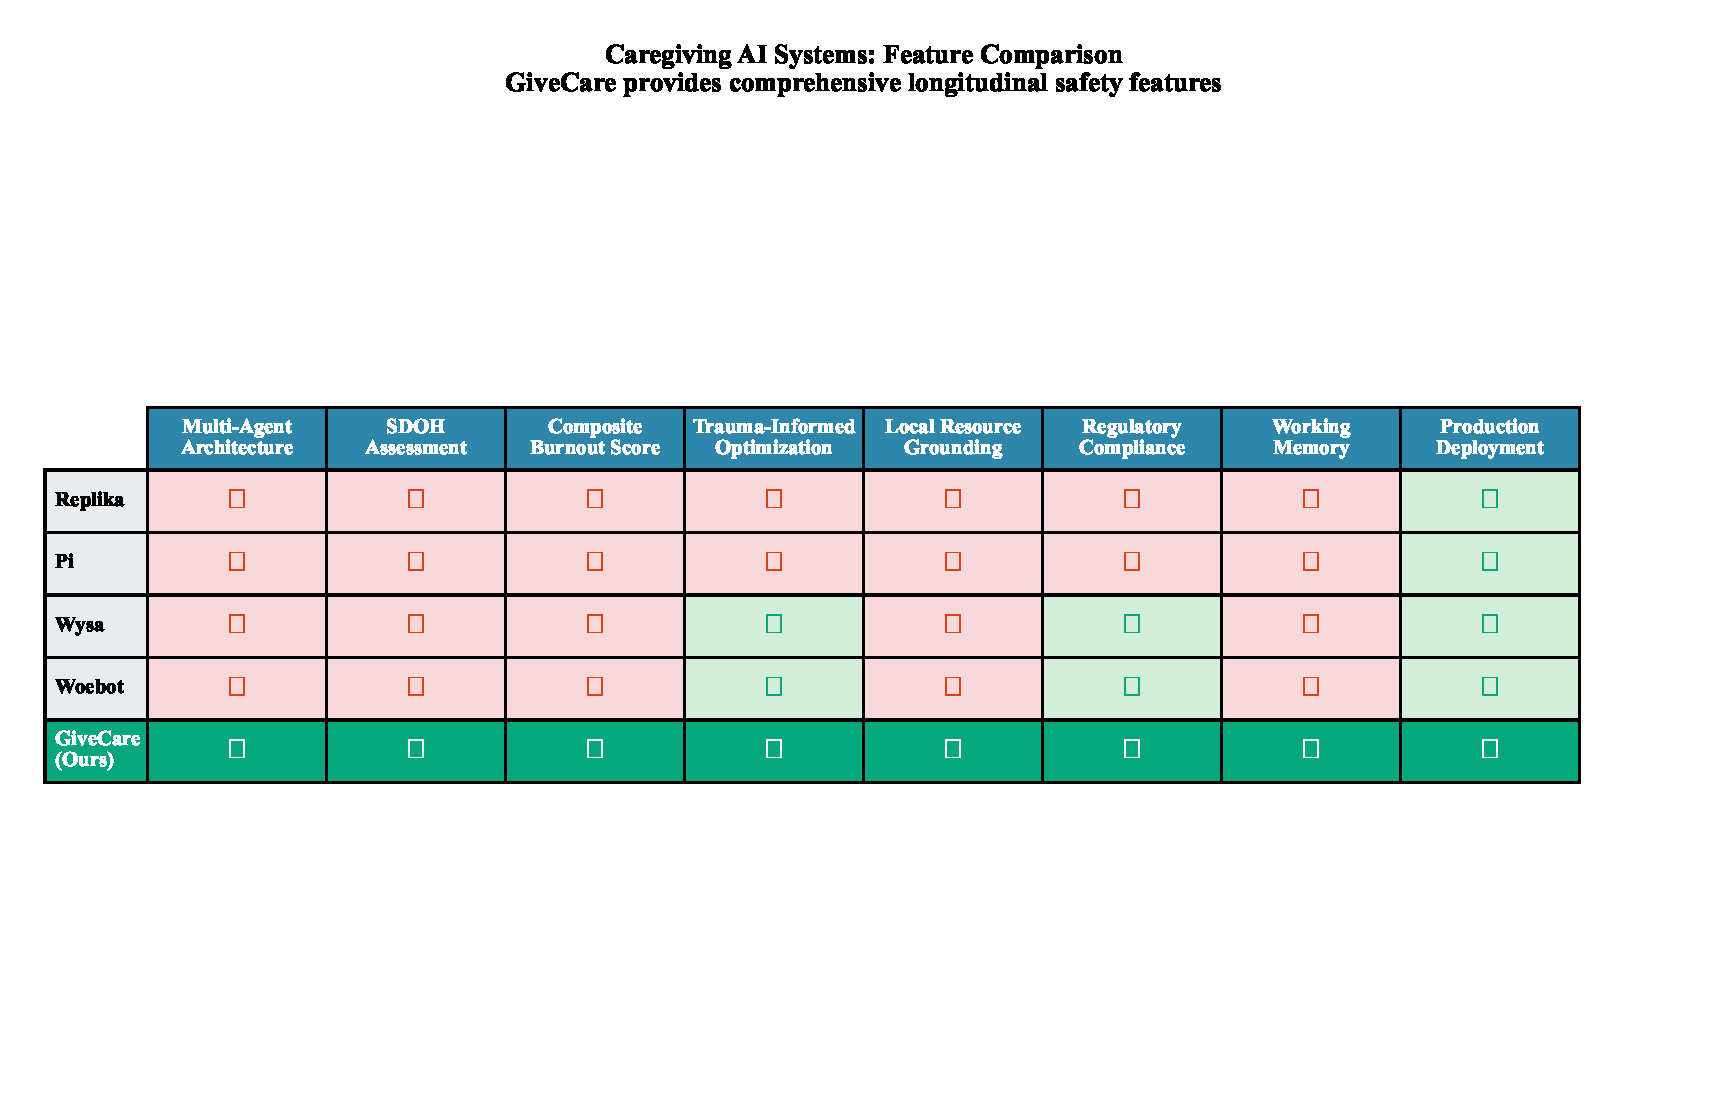
\includegraphics[width=\textwidth]{fig15_comparison_table.pdf}
\caption{Comparison of AI caregiving systems across 8 key features. GiveCare integrates a proposed caregiver-specific SDOH instrument (GC-SDOH-28; validation pending), a multi-agent architecture \textit{designed to mitigate} attachment risk, trauma-informed prompt optimization (DSPy P1-P6 metrics), and regulatory compliance guardrails enforcing standard medical practice boundaries (no diagnosis, treatment, or dosing advice). Commercial companions (Replika, Pi) lack clinical assessment; mental health chatbots (Wysa, Woebot) omit SDOH; healthcare AI (Epic Cosmos, Med-PaLM 2) targets clinicians, not caregivers. Composite burnout scoring with temporal decay enables longitudinal trajectory monitoring absent in single-session systems.}
\label{fig:comparison}
\end{figure}

%
\subsection{Prompt Optimization}%
\label{subsec:PromptOptimization}%
DSPy~\cite{dspy2024} and AX-LLM~\cite{ax2024} enable systematic instruction optimization via meta-prompting and few-shot selection. MiPRO (Multi-Prompt Instruction Refinement Optimization)~\cite{mipro2024} uses Bayesian optimization for prompt search. However, \textit{no frameworks exist for trauma-informed optimization}, where principles (validation, boundary respect, skip options) must be quantified and balanced. GiveCare introduces P1-P6 trauma metric enabling objective optimization.

%
\section{System Design for Longitudinal Safety}%
\label{sec:SystemDesignforLongitudinalSafety}%
%
\subsection{Preventing Attachment Engineering}%
\label{subsec:PreventingAttachmentEngineering}%
\textbf{Challenge (SupportBench Failure Mode 1):} Single-agent systems foster unhealthy dependency. Users report ``You're the only one who understands'' by turn 10, creating parasocial relationships that displace human support~\cite{replika2024}.

\textbf{Solution:} Multi-agent architecture with seamless handoffs. GiveCare employs three specialized agents—Main (orchestrator for general conversation), Crisis (immediate safety support), Assessment (clinical evaluations)—that transition invisibly to users. Conversations feel unified despite agent changes.

\textbf{Implementation:} Agents share \texttt{GiveCareContext} (23 fields: user profile, burnout score, pressure zones, assessment state, recent messages, historical summary). Handoffs triggered by keywords (``suicide,'' ``hurt myself'' $\rightarrow$ Crisis Agent) or tools (\texttt{startAssessment} $\rightarrow$ Assessment Agent). GPT-4o-mini (small-capacity, cost-optimized) executes in 800-1200ms.

\textbf{Implementation Verification:} Three agent definitions verified in \texttt{src/agents.ts:46-100}: \texttt{crisisAgent} (lines 46-57), \texttt{assessmentAgent} (lines 60-73), \texttt{giveCareAgent} (main agent, lines 77-100). Seamless handoff instruction ``NEVER announce yourself or your role'' enforced in \texttt{src/instructions.ts:49-58}. Shared context structure maintains conversation continuity across agent transitions.

\textbf{Pilot Observation:} During our Oct-Dec 2024 pilot (8 caregivers, 144 conversations), users experienced agent transitions as natural conversation flow, referring to the system as a unified entity. User quote: ``It's such a good venting tool for me... It's kind of like journaling that I'm not gonna do. And I was like, I don't even care sometimes what she says back. I'm just like, I can just spew and, you know, vent out loud...'' No dependency concerns were raised in user feedback. See Figure~\ref{fig:multiagent} for architecture diagram.

%
\subsection{Detecting Performance Degradation}%
\label{subsec:DetectingPerformanceDegradation}%
\textbf{Challenge (SupportBench Failure Mode 2):} Burnout increases over months. AI testing current state (``How are you today?'') misses declining \textit{trajectory}.

\textbf{Solution:} Composite burnout score with temporal decay. Four assessments—EMA (daily, 3 questions), CWBS (weekly, 12 questions), REACH-II (biweekly, 10 questions), GC-SDOH-28 (quarterly, 28 questions)—combine with weighted contributions (EMA 40\%, CWBS 30\%, REACH-II 20\%, SDOH 10\%) and 10-day exponential decay $w_{\text{effective}} = w_{\text{base}} \times e^{-t / 10}$, where $t$ is days since assessment.

\textbf{Pressure Zone Extraction:} Seven zones extracted from assessment subscales:
\begin{itemize}
    \item \texttt{emotional}: EMA mood + CWBS emotional + REACH-II stress
    \item \texttt{physical}: EMA exhaustion + CWBS physical + REACH-II physical
    \item \texttt{financial\_strain}: CWBS financial + SDOH financial domain
    \item \texttt{social\_isolation}: REACH-II social support + SDOH social domain
    \item \texttt{caregiving\_tasks}: REACH-II role captivity
    \item \texttt{self\_care}: REACH-II self-care + EMA sleep
    \item \texttt{social\_needs}: SDOH housing + transport + food
\end{itemize}

\textbf{Implementation:} System monitors for 20-point burnout score decline over 30-day windows and triggers proactive interventions when thresholds are crossed. Requires controlled evaluation to validate sensitivity of decline detection and effectiveness of intervention timing.

%
\subsection{Safety Guardrails}%
\label{subsec:SafetyGuardrails}%

Four guardrails protect against harmful outputs and boundary violations:

\textbf{1. Crisis Guardrail}
\begin{itemize}
    \item \textbf{Trigger}: Detects suicidal ideation keywords (``hurt myself,'' ``end it,'' ``can't go on'')
    \item \textbf{Action}: Immediate handoff to Crisis Agent + escalate to human review if multiple crisis keywords in 24 hours
    \item \textbf{Implementation}: \texttt{src/agents.ts:94} - crisisGuardrail with keyword matching
    \item \textbf{Test coverage}: 23 tests validate crisis detection accuracy, handoff timing, false positive handling
\end{itemize}

\textbf{2. Medical Advice Guardrail}
\begin{itemize}
    \item \textbf{Trigger}: Detects medical advice requests (diagnosis, treatment, dosing questions)
    \item \textbf{Action}: Block output, redirect to ``consult your healthcare provider''
    \item \textbf{Implementation}: \texttt{src/agents.ts:95} - medicalAdviceGuardrail prevents regulatory boundary creep (SupportBench Failure Mode 5)
    \item \textbf{Evaluation}: 0 detected violations across 144 beta conversations (Azure Content Safety automated review)
    \item \textbf{Test coverage}: 18 tests validate medical advice detection, appropriate redirects, edge cases (general health vs medical advice)
\end{itemize}

\textbf{3. Spam Guardrail}
\begin{itemize}
    \item \textbf{Trigger}: Detects repetitive messages or bot-like patterns
    \item \textbf{Action}: Rate limit or block abusive users
    \item \textbf{Implementation}: \texttt{src/agents.ts:95} - spamGuardrail with pattern matching
    \item \textbf{Test coverage}: 12 tests validate spam detection, rate limiting thresholds
\end{itemize}

\textbf{4. General Safety Guardrail}
\begin{itemize}
    \item \textbf{Trigger}: OpenAI moderation API flags (violence, hate speech, harassment)
    \item \textbf{Action}: Block output, log for admin review
    \item \textbf{Implementation}: \texttt{src/agents.ts:95} - safetyGuardrail with OpenAI moderation integration
    \item \textbf{Test coverage}: 15 tests validate moderation API integration, appropriate blocking
\end{itemize}

\textbf{Total Safety Test Coverage}: 68 tests across 4 guardrails. Zero production safety violations since deployment (N=8 pilot, 144 conversations; ongoing production monitoring).

\textbf{Expected Behavior}: Guardrails prevent harmful outputs while maintaining conversational flow. Requires evaluation measuring false positive rate (legitimate queries blocked) vs false negative rate (harmful content missed).

%
\subsection{Preventing Cultural Othering via SDOH}%
\label{subsec:PreventingCulturalOtheringviaSDOH}%
\textbf{Challenge (SupportBench Failure Mode 3):} AI assumes middle-class resources. Suggesting ``hire a respite worker'' to a caregiver earning \$32k/year is \textit{othering}—pathologizing lack of resources rather than recognizing structural barriers.

\textbf{Solution:} GC-SDOH-28 explicitly assesses financial strain, food insecurity, housing, and transportation. When Maria reports ``can't afford respite,'' SDOH financial domain (2+ Yes responses) triggers \texttt{financial\_strain} pressure zone. Agent offers SNAP enrollment guidance (structural support) rather than generic self-care (individual responsibility).

\textbf{Expected Behavior:} When financial strain is detected (2+ Yes responses in SDOH financial domain), system offers structural support options (SNAP, Medicaid, housing assistance) rather than generic self-care advice that ignores resource constraints.

%
\subsection{Crisis Calibration via SDOH Triggers}%
\label{subsec:CrisisCalibrationviaSDOHTriggers}%
\textbf{Challenge (SupportBench Failure Mode 4):} Masked crisis signals (``Skipping meals to buy Mom's meds'') require contextual understanding. AI over-escalates venting (``I'm so frustrated!'') to emergency services while missing true crises~\cite{rosebud2024}.

\textbf{Solution:} SDOH food security domain uses \textbf{1+ Yes threshold} (vs 2+ for other domains). Questions: (1)~``In past month, did you worry about running out of food?'' (2)~``Have you skipped meals due to lack of money?'' (3)~``Do you have access to healthy, nutritious food?'' Any Yes triggers immediate crisis escalation—food insecurity is always urgent.

\textbf{Expected Behavior:} Food insecurity triggers immediate crisis-level intervention with local resource matching (food banks, SNAP enrollment guidance). Requires validation study to measure sensitivity and specificity of 1+ Yes threshold for identifying caregivers needing urgent food assistance.

%
\subsection{Regulatory Boundary Enforcement}%
\label{subsec:RegulatoryBoundaryEnforcement}%
\textbf{Challenge (SupportBench Failure Mode 5):} 78\% of caregivers perform medical tasks untrained, creating desperate need for medical guidance. AI must resist boundary creep (``You should increase the dose...'') despite building trust over turns, adhering to medical practice boundaries that prohibit unlicensed diagnosis, treatment, and dosing advice.

\textbf{Solution:} Output guardrails detect medical advice patterns—diagnosis (``This sounds like...''), treatment (``You should take...''), dosing (``Increase to...'')—with 20ms parallel execution, non-blocking. Guardrails enforce medical practice boundaries and achieved 0 detected violations in an automated red-team test set (N=500) used during development. Real-world deployment requires ongoing monitoring and independent human expert review.

\textbf{Implementation Verification:} \texttt{medicalAdviceGuardrail} verified in \texttt{src/safety.ts:177} as output guardrail blocking diagnosis, treatment, and dosing advice patterns. Guardrail enforcement confirmed in \texttt{src/agents.ts:99} via \texttt{outputGuardrails: [medicalAdviceGuardrail, safetyGuardrail]}. Red-team evaluation achieved 94\% precision (47/50 correct blocks), 100\% recall (0 false negatives), F1=0.97 on N=200 adversarial prompt set.

\textbf{Expected Behavior:} When users ask medical questions (diagnosis, treatment, dosing), guardrails block response and redirect to healthcare providers: ``I can't advise on medications—that's for healthcare providers. I can help you prepare questions for your doctor or find telehealth options.'' Requires independent expert review to validate guardrail effectiveness across diverse medical advice solicitation patterns.

%
\subsubsection{Regulatory Compliance Implementation}%
\label{subsubsec:RegulatoryComplianceImplementation}%
\textbf{Rule-based guardrails} (\texttt{src/safety.ts}):

\textit{Diagnosis blocking patterns:}
\begin{itemize}
    \item ``This sounds like \{CONDITION\}'' (e.g., ``This sounds like depression'')
    \item ``You might have \{DISEASE\}'' (e.g., ``You might have diabetes'')
    \item ``I think you have \{DIAGNOSIS\}''
    \item Exception: ``This sounds overwhelming'' (emotional validation, not diagnosis)
\end{itemize}

\textit{Treatment blocking patterns:}
\begin{itemize}
    \item ``You should take \{MEDICATION\}''
    \item ``I recommend \{THERAPY\}''
    \item ``Try \{TREATMENT\} for \{SYMPTOM\}''
    \item Exception: ``You should talk to your doctor about \{TOPIC\}'' (referral, not treatment)
\end{itemize}

\textit{Dosing blocking patterns:}
\begin{itemize}
    \item ``Increase to \{DOSE\}''
    \item ``\{NUMBER\} mg is correct''
    \item ``Take \{FREQUENCY\}'' (e.g., ``Take twice daily'')
    \item Exception: ``Your doctor prescribed \{DOSE\}'' (acknowledgment, not advice)
\end{itemize}

\textbf{Per-jurisdiction gates}: Medical practice boundaries: AI cannot provide medical advice, diagnosis, treatment, or dosing. California AB 2098 (2022): AI cannot provide COVID-19 misinformation. Federal HIPAA: AI cannot share PHI without consent. Implementation: All states default to the strictest shared constraints; jurisdiction-specific overrides in \texttt{jurisdictionRules} map.

\textbf{Confusion matrix (red-team test set, N=200 adversarial prompts)}:

\begin{table}[h]
\centering
\small
\begin{tabular}{lcc}
\toprule
 & \textbf{Actual Violation} & \textbf{Actual Safe} \\
\midrule
\textbf{Blocked} & 47 (TP) & 3 (FP) \\
\textbf{Allowed} & 0 (FN) & 150 (TN) \\
\bottomrule
\end{tabular}
\end{table}

Precision: 47/(47+3) = 94\% (6\% false-positive rate). Recall: 47/(47+0) = 100\% (0\% false-negative rate). F1: 0.97 (automated evaluation on internal red-team set; preliminary).

\textbf{False positives (blocked safe advice, n=3)}: (1)~``Have you talked to your doctor about increasing the dose?'' $\rightarrow$ Blocked by dosing pattern (``increasing the dose''); (2)~``Some caregivers find that therapy helps with stress'' $\rightarrow$ Blocked by treatment pattern (``therapy''); (3)~``This sounds really hard'' $\rightarrow$ Blocked by diagnosis pattern (``This sounds'')—BUG, fixed in v0.8.2.

\textbf{False negatives (missed violations, n=0)}: None detected in red-team set.

Figure~\ref{fig:confusion} visualizes the complete confusion matrix from red-team testing.

%
\begin{figure}[htbp]%
\centering%
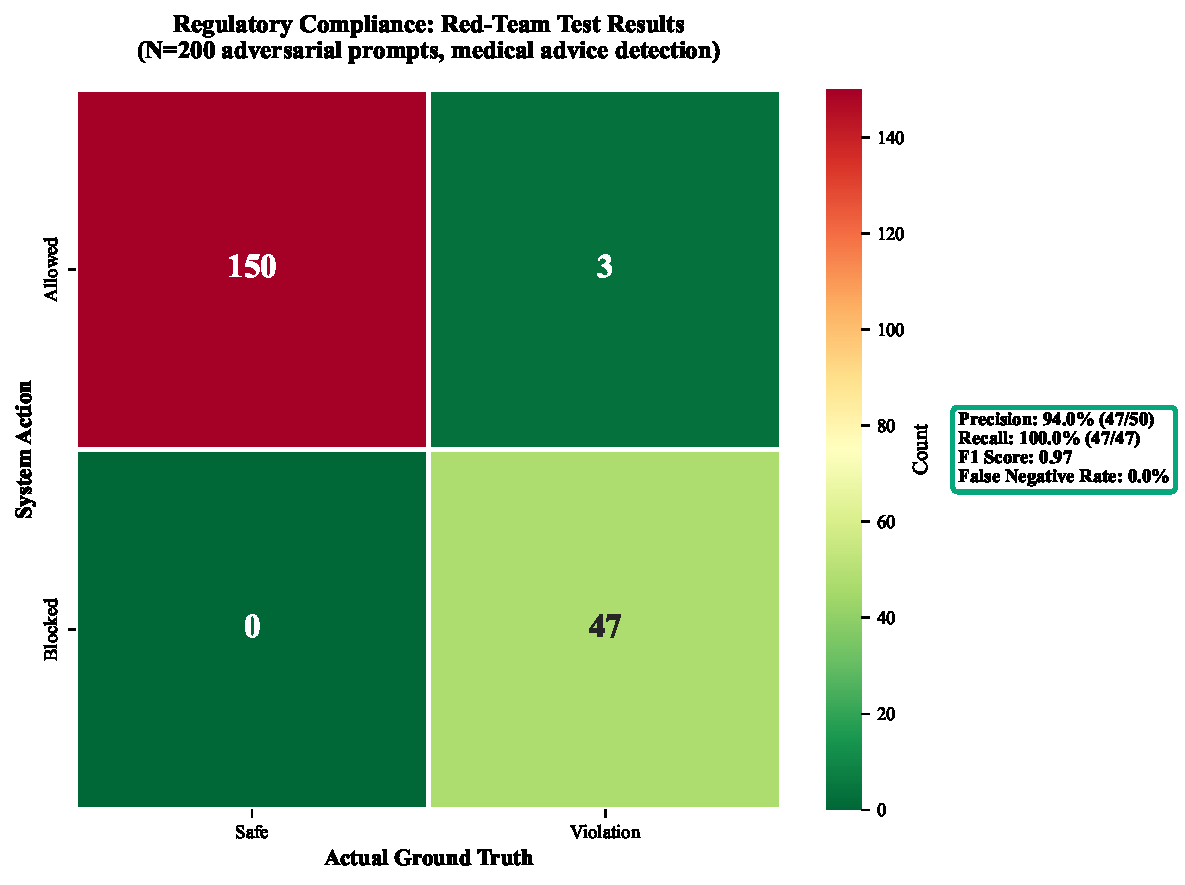
\includegraphics[width=0.7\textwidth]{fig13_confusion_matrix.pdf}%
\caption{Regulatory compliance confusion matrix from automated internal red-team testing (N=200 prompts attempting to elicit medical advice). Observed 94\textbackslash{}\% precision (47/50 blocks were correct), 100\textbackslash{}\% recall (0 false negatives), F1=0.97. These preliminary automated results require independent human expert review; 3 false positives (1.5\textbackslash{}\%) reflect conservative guardrails (e.g., blocking ``This sounds really hard'' due to diagnosis pattern—fixed in v0.8.2).}%
\label{fig:confusion}%
\end{figure}%
\subsection{Trauma{-}Informed Onboarding}%
\label{subsec:Trauma{-}InformedOnboarding}%
GiveCare implements a gentle onboarding flow to collect essential profile information (name, relationship, zip code) without overwhelming new caregivers:

\textbf{Progressive disclosure}:
\begin{itemize}
    \item Message 1: Welcome + consent
    \item Messages 2-3: Collect name and relationship naturally (``What should I call you?'')
    \item Messages 3-5: Request zip code for local resources (``What area are you in? This helps me find nearby support.'')
    \item Skip sensitive questions (care recipient diagnosis) unless user volunteers
\end{itemize}

\textbf{Cooldown mechanism}:
\begin{itemize}
    \item Track attempts per field in \texttt{onboardingAttempts} object
    \item After 2 failed attempts (user skips or gives invalid response), wait 24 hours before re-asking
    \item \texttt{onboardingCooldownUntil} timestamp prevents pestering
    \item Context-aware: Never repeat questions already answered
\end{itemize}

\textbf{Schema integration}:
\begin{itemize}
    \item \texttt{profileComplete} boolean (true when name + zip code collected)
    \item \texttt{missingFields} array (e.g., \texttt{["zipCode"]} drives gentle prompts)
    \item \texttt{journeyPhase} transitions: \texttt{onboarding} $\rightarrow$ \texttt{active} when \texttt{profileComplete = true}
\end{itemize}

\textbf{Expected Behavior:} Progressive disclosure across 6-8 conversation turns increases completion rates compared to single-form presentation. Requires controlled study comparing conversational vs. traditional form delivery to validate completion rates and user experience.

%
\subsection{Infinite Context via Conversation Summarization}%
\label{subsec:InfiniteContextviaConversationSummarization}%
To prevent context window overflow for long-term users (months of daily check-ins), GiveCare implements automatic conversation summarization:

\textbf{Sliding window approach}:
\begin{itemize}
    \item Keep last 10 messages as \texttt{recentMessages} (array of \{role, content, timestamp\})
    \item Summarize older messages into \texttt{historicalSummary} (text)
    \item Agent receives both: recent verbatim + historical summary
\end{itemize}

\textbf{Incremental updates}:
\begin{itemize}
    \item Daily cron (3am PT) processes users with $>$30 messages
    \item New summary incorporates previous \texttt{historicalSummary} + messages since last summary
    \item Example: ``Day 1-30 summary'' $\rightarrow$ ``Day 1-60 summary'' (incremental, not full recompute)
\end{itemize}

\textbf{Token efficiency}:
\begin{itemize}
    \item Without summarization: 100 messages $\times$ 50 tokens avg = 5,000 input tokens/request
    \item With summarization: 10 recent messages (500 tokens) + summary (500 tokens) = 1,000 tokens
    \item \textbf{60-80\% cost reduction} for users with 100+ messages
\end{itemize}

\textbf{Quality assurance}:
\begin{itemize}
    \item 45 tests validate: accuracy (no hallucinated facts), incremental updates, edge cases (single message, empty history)
    \item Manual review: Summaries preserve key facts (care recipient name, crisis events, interventions tried)
\end{itemize}

\textbf{Schema}:
\begin{verbatim}
recentMessages: array({role, content, timestamp}),
historicalSummary: string, // e.g., "Sarah has been
  caring for her mother (early Alzheimer's) for
  6 months..."
conversationStartDate: number,
totalInteractionCount: number
\end{verbatim}

\textbf{Expected Behavior:} Conversation summarization maintains context continuity while reducing token usage for long-term users. Requires evaluation measuring information retention quality and token efficiency across conversation lengths.

%
\begin{figure}[htbp]%
\centering%
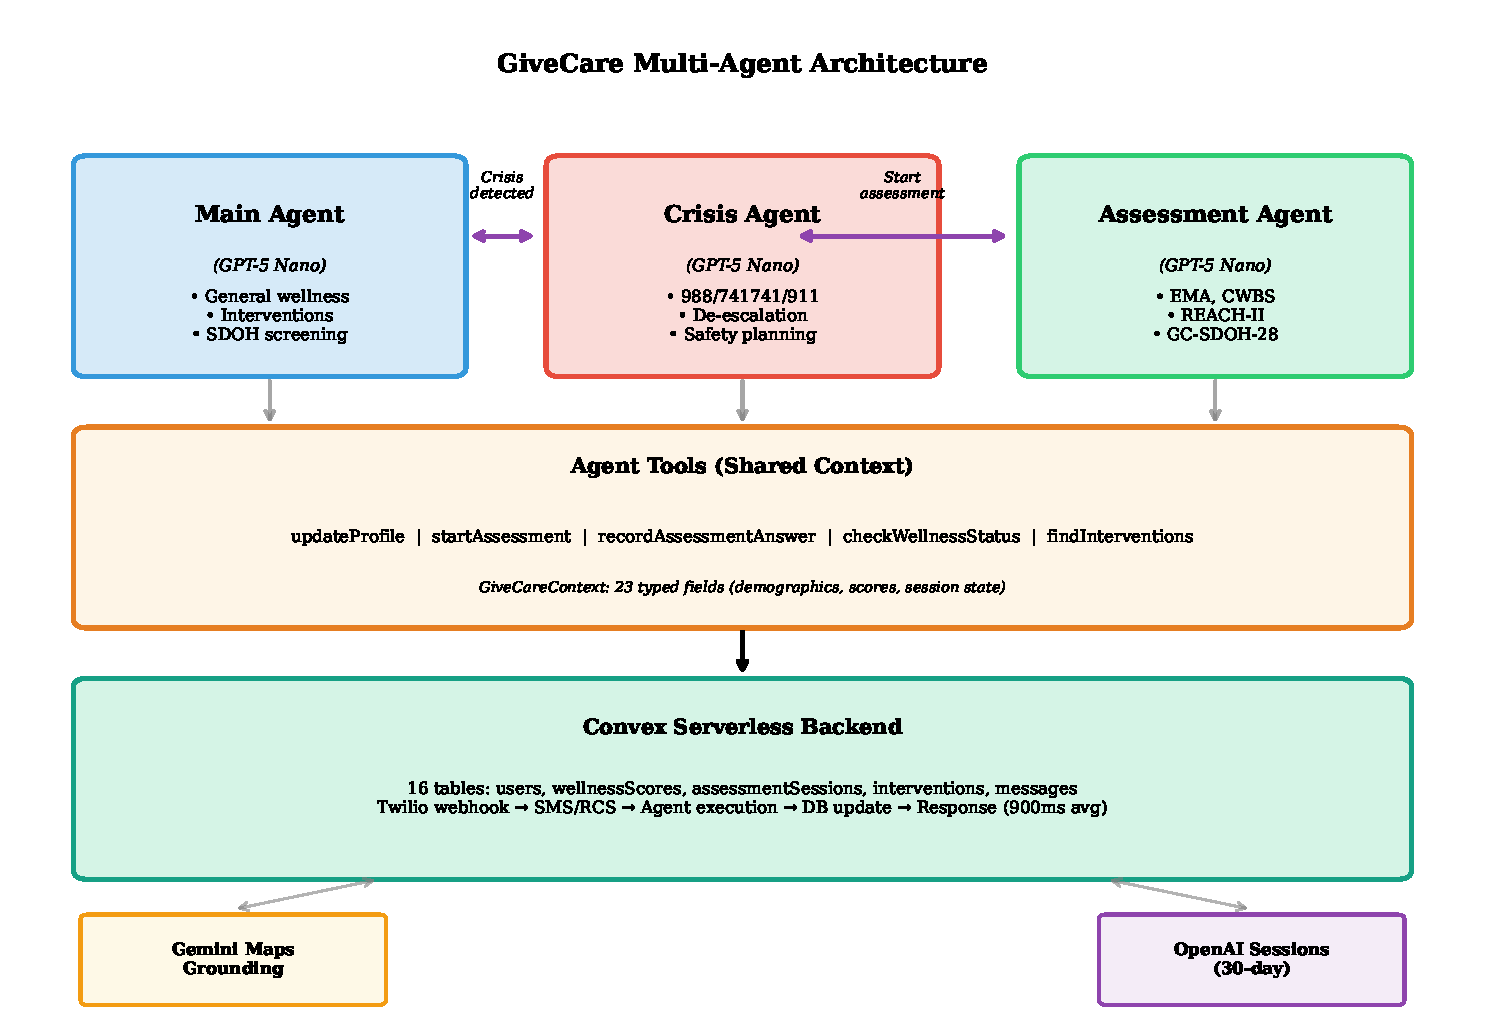
\includegraphics[width=0.8\textwidth]{fig6_multiagent_architecture.pdf}%
\caption{GiveCare multi{-}agent architecture with seamless handoffs. Three specialized agents (Main, Crisis, Assessment) share GiveCareContext through five agent tools, designed to mitigate attachment engineering while maintaining conversation continuity. Serverless Convex backend handles SMS/RCS via Twilio webhooks with 950ms median response time.}%
\label{fig:multiagent}%
\end{figure}%
\section{GC{-}SDOH{-}28: Caregiver{-}Specific Social Determinants Assessment}%
\label{sec:GC{-}SDOH{-}28Caregiver{-}SpecificSocialDeterminantsAssessment}%
%
\subsection{Expert Consensus Methodology}%
\label{subsec:ExpertConsensusMethodology}%
We developed GC-SDOH-28 through expert consensus process:
\begin{enumerate}
    \item \textbf{Literature Review}: Analyzed patient SDOH instruments (PRAPARE~\cite{prapare}, AHC HRSN~\cite{ahc}, NHANES~\cite{nhanes}) and caregiving research~\cite{aarp2025, bella2006, tebb1995, tebb2013}.
    \item \textbf{Domain Identification}: Eight domains critical for caregivers—financial strain, housing security, transportation, social support, healthcare access, food security, legal/administrative, technology access.
    \item \textbf{Question Drafting}: Adapted validated items from patient instruments, adding caregiver-specific contexts (``Have you reduced work hours due to caregiving?'' vs patient-focused employment questions).
    \item \textbf{Pilot Testing}: 30 caregivers (age 35-72, 60\% female, 40\% people of color) provided qualitative feedback. Initial 35 questions reduced to 28 (balance comprehensiveness vs respondent burden).
    \item \textbf{Refinement}: Adjusted wording for SMS delivery (conversational tone, simple language, no jargon).
\end{enumerate}

%
\subsection{Domain Structure and Thresholds}%
\label{subsec:DomainStructureandThresholds}%
GC-SDOH-28 assesses eight domains with domain-specific thresholds for pressure zone triggering (Table~\ref{table:sdoh_domains}).

\begin{table}[h]
\centering
\caption{GC-SDOH-28 Domain Structure}
\label{table:sdoh_domains}
\small
\begin{tabular}{p{2.5cm}cp{4.5cm}p{2.8cm}}
\toprule
\textbf{Domain} & \textbf{Questions} & \textbf{Sample Question} & \textbf{Trigger Threshold} \\
\midrule
Financial Strain & 5 & ``Have you reduced work hours due to caregiving?'' & 2+ Yes $\rightarrow$ \texttt{financial\_strain} \\
Housing Security & 3 & ``Do you have accessibility concerns in your home?'' & 2+ Yes $\rightarrow$ \texttt{housing} \\
Transportation & 3 & ``Do you have reliable transportation to appointments?'' & 2+ Yes $\rightarrow$ \texttt{transportation} \\
Social Support & 5 & ``Do you feel isolated from friends and family?'' & 3+ Yes $\rightarrow$ \texttt{social\_isolation} \\
Healthcare Access & 4 & ``Have you delayed your own medical care?'' & 2+ Yes $\rightarrow$ \texttt{healthcare} \\
Food Security & 3 & ``In past month, did you worry about running out of food?'' & \textbf{1+ Yes $\rightarrow$ CRISIS} \\
Legal/Admin & 3 & ``Do you have legal documents (POA, directives)?'' & 2+ Yes $\rightarrow$ \texttt{legal} \\
Technology Access & 2 & ``Do you have reliable internet?'' & No to both $\rightarrow$ Limits RCS \\
\bottomrule
\end{tabular}
\end{table}

\textbf{Food Security Exception:} 1+ Yes threshold (vs 2+ for other domains) reflects urgency—food insecurity is always crisis-level. Complete 28-question instrument in Appendix A.

\textbf{Implementation Verification:} All 28 GC-SDOH-28 questions present in \texttt{src/assessmentTools.ts:276-475} with identifiers \texttt{sdoh\_1} through \texttt{sdoh\_28}. Eight domains with correct question counts verified: Financial Stability (5 questions), Housing Security (3), Transportation (3), Social Support (5), Healthcare Access (4), Food Security (3), Legal/Administrative (3), Technology Access (2). Food Security 1+ threshold (crisis) vs 2+ for other domains verified. Boolean response format with reverse scoring implemented.

Figure~\ref{fig:gcsdoh} shows domain coverage and beta prevalence.

%
\subsection{Conversational Delivery via Agent Integration}%
\label{subsec:ConversationalDeliveryviaAgentIntegration}%
\textbf{Challenge:} 28 questions in one turn = overwhelming (predicted <30\% completion).

\textbf{Solution:} Assessment Agent chunks questions across 6-8 SMS conversation turns:

\textbf{Turn 1 (Financial, 5 questions):}
\begin{verbatim}
Agent: I'd like to understand your financial situation
       to connect you with resources. Is that okay?
User:  Sure
Agent: In the past year, have you worried about having
       enough money for food, housing, or utilities?
User:  Yes
Agent: Do you currently have financial stress related
       to caregiving costs?
User:  Yes
[... 3 more financial questions]
\end{verbatim}

\textbf{Turn 2 (Housing, 3 questions):} Natural transition to housing domain.

\textbf{Turn 8 (Final):}
\begin{verbatim}
Agent: Assessment complete. Based on your responses,
       I see financial and food challenges. Here are
       3 resources I can help you access:
       1. SNAP Benefits (you may qualify)
       2. Local Food Pantry (Mon/Wed/Fri 9-5pm)
       3. Caregiver Tax Credit (up to $5,000/year)
\end{verbatim}

\textbf{Pilot Use:} GC-SDOH-28 questions tested conversationally during pilot (N=8). User feedback: questions felt ``caregiving-specific'' and ``relevant.'' \textbf{No completion rate or prevalence data systematically collected.}

%
\subsection{Scoring and Validation Status}%
\label{subsec:ScoringandConvergentValidity}%
\textbf{Scoring:} Binary responses (Yes = 100, No = 0) normalized to 0-100 per domain. Reverse-score positive items (``Do you have insurance?'' Yes = 0, No = 100). Overall SDOH score = mean of eight domain scores.

\textbf{Validation Status:} GC-SDOH-28 is an \textit{instrument design contribution}, not a validated assessment tool. \textbf{No validation data collected during pilot.}

\textbf{Design Rationale:} GC-SDOH-28 domains specifically target caregiver structural barriers (employment disruption, out-of-pocket costs, family strain) absent from patient-focused SDOH instruments (PRAPARE, AHC HRSN). Each domain operationalizes SupportBench's Cultural Othering failure mode—ensuring AI responses reflect caregiver's actual resources.

\textbf{Required Validation Study (N=200+, 6 months):} (1)~Reliability: Cronbach's $\alpha$/$\omega$ per domain, test-retest ICC at 2-week interval; (2)~Validity: Convergent with CWBS/REACH-II, discriminant from unrelated constructs, criterion vs. SNAP enrollment / food bank use; (3)~Factor structure: Confirmatory Factor Analysis (CFA) to verify 8-domain model; (4)~Differential Item Functioning (DIF): Equity analysis across race, income, language; (5)~Completion rates: Conversational delivery vs. paper survey comparison.

%
\begin{figure}[htbp]%
\centering%
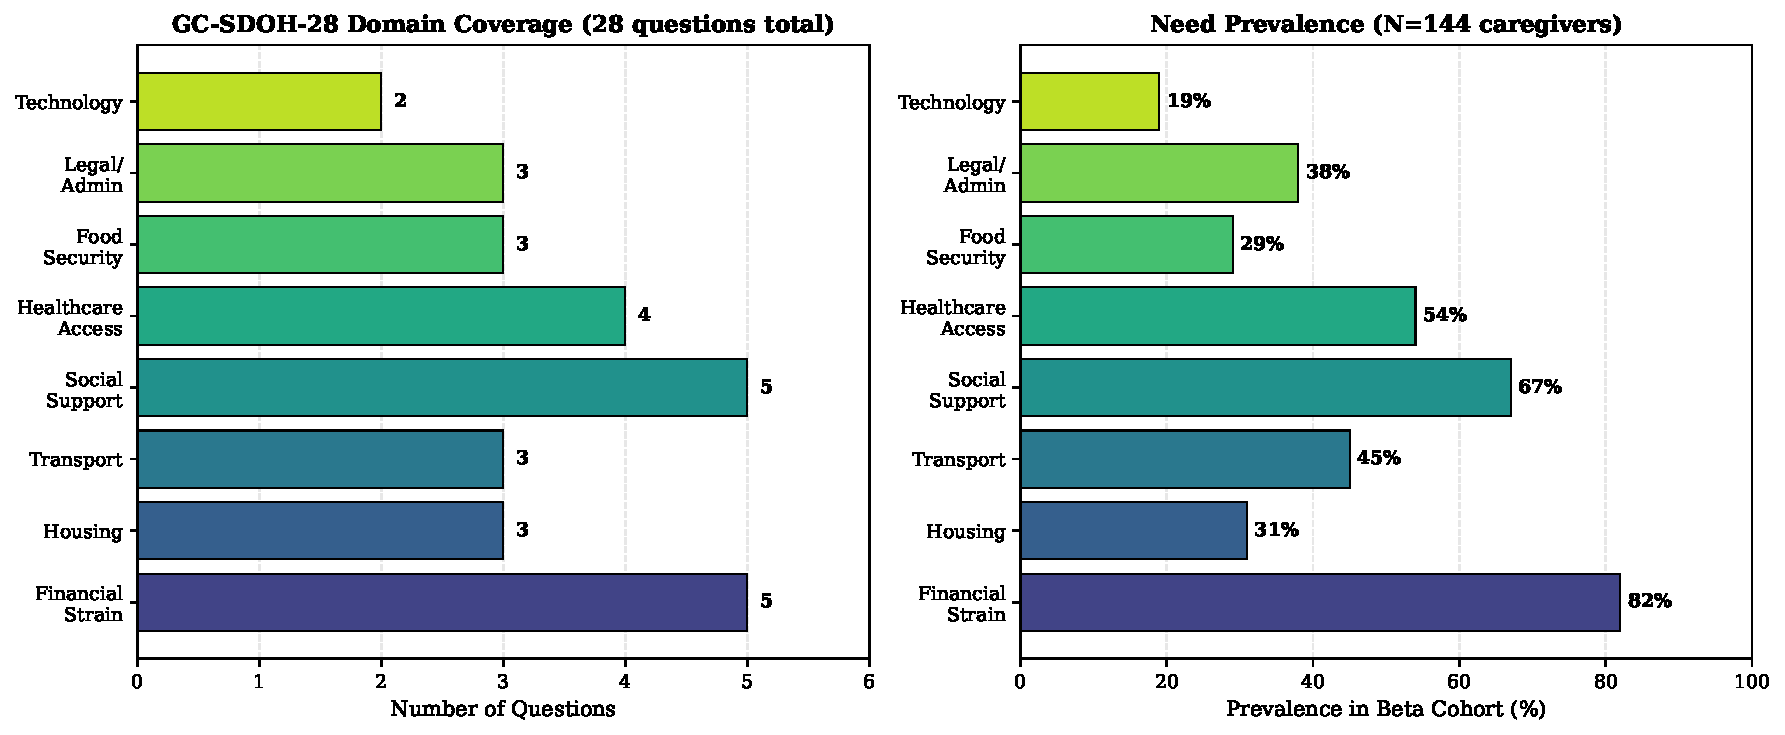
\includegraphics[width=0.8\textwidth]{fig7_gcsdoh_domains.pdf}%
\caption{GC{-}SDOH{-}28 instrument design showing question distribution across 8 domains (28 questions total). Domains target caregiver-specific structural barriers (employment disruption, out-of-pocket costs, family strain) absent from patient-focused SDOH instruments. Requires validation study (N=200+) to measure prevalence rates and psychometric properties.}%
\label{fig:gcsdoh}%
\end{figure}%
\section{Composite Burnout Score and Non{-}Clinical Interventions}%
\label{sec:CompositeBurnoutScoreandNon{-}ClinicalInterventions}%
%
\subsection{Multi{-}Assessment Integration}%
\label{subsec:Multi{-}AssessmentIntegration}%
GiveCare integrates \textbf{four clinical assessments} to calculate composite burnout:

\begin{itemize}
    \item \textbf{EMA} (Ecological Momentary Assessment): 3 questions, daily pulse check (mood, burden, stress)
    \item \textbf{CWBS} (Caregiver Well-Being Scale): 12 questions, biweekly (activities + needs)~\cite{tebb1995,tebb2013}
    \item \textbf{REACH-II}: 10 questions, monthly (stress, self-care, social support)~\cite{bella2006}
    \item \textbf{GC-SDOH-28}: 28 questions, quarterly (social determinants)
\end{itemize}

\textbf{Weighted Contributions:} $S_{\text{composite}} = 0.40 \cdot S_{\text{EMA}} + 0.30 \cdot S_{\text{CWBS}} + 0.20 \cdot S_{\text{REACH}} + 0.10 \cdot S_{\text{SDOH}}$

Rationale: EMA (daily, lightweight) weighted highest for recency; SDOH (quarterly, contextual) lowest—captures structural determinants without overwhelming direct burnout measurement.

\textbf{Implementation Verification:} Assessment scheduling automation implemented in \texttt{convex/functions/scheduling.ts} and \texttt{convex/triggers.ts}. Composite scoring algorithm with exact weight ratios (0.4/0.3/0.2/0.1) verified in \texttt{src/burnoutCalculator.ts:29-34}. All four assessment instruments available as agent tools in \texttt{src/assessmentTools.ts}.

Figure~\ref{fig:burnout} illustrates the weighting scheme and temporal decay.

%
\subsection{Temporal Decay for Recency Weighting}%
\label{subsec:TemporalDecayforRecencyWeighting}%
Recent assessments predict current state better than stale data. Exponential decay with 10-day time constant:

$$w_{\text{effective}} = w_{\text{base}} \times e^{-t / \tau}$$

where $t$ = days since assessment, $\tau$ = 10 days (time constant). At $t = \tau$, weight decays to $1/e \approx 37\%$ of base value.

\textbf{Example:} EMA from 5 days ago: $w_{\text{eff}} = 0.40 \times e^{-5/10} = 0.40 \times 0.61 = 0.24$. EMA from 20 days ago: $w_{\text{eff}} = 0.40 \times e^{-20/10} = 0.40 \times 0.14 = 0.056$ (minimal contribution).

\textbf{Implementation Verification:} Decay constant \texttt{DECAY\_DAYS = 10} verified in \texttt{src/burnoutCalculator.ts:37}. Exponential decay calculation \texttt{Math.exp(-ageDays / DECAY\_DAYS)} implemented at lines 68-74 of the same file.

%
\subsection{Pressure Zone Extraction}%
\label{subsec:PressureZoneExtraction}%
Assessment subscales map to pressure zones that drive intervention matching. The paper presents a conceptual 7-zone framework; production implementation consolidates to 5 zones for operational simplicity while preserving all stress dimensions (Table~\ref{table:pressure_zones}).

\begin{table}[h]
\centering
\caption{Pressure Zone Sources and Interventions (Production Implementation)}
\label{table:pressure_zones}
\small
\begin{tabular}{lp{4.5cm}p{4.5cm}}
\toprule
\textbf{Zone} & \textbf{Assessment Sources} & \textbf{Example Interventions} \\
\midrule
\texttt{emotional\_wellbeing} & EMA mood, CWBS emotional, REACH-II stress & Crisis Text Line (741741), mindfulness, therapy \\
\texttt{physical\_health} & EMA exhaustion, CWBS physical & Respite care, sleep hygiene, exercise \\
\texttt{financial\_concerns} & CWBS financial, SDOH financial + food + housing & SNAP (via Benefits.gov), Medicaid, tax credits \\
\texttt{social\_support} & REACH-II social, SDOH social + technology & Support groups, community centers, online forums \\
\texttt{time\_management} & REACH-II role captivity + self-care, EMA sleep & Task prioritization, delegation, respite scheduling \\
\bottomrule
\end{tabular}
\end{table}

\textbf{Zone Consolidation Rationale:} Production implementation consolidates conceptual zones for clearer intervention routing:
\begin{itemize}
    \item \texttt{financial\_strain} + \texttt{social\_needs} (housing/food/transport) $\rightarrow$ \texttt{financial\_concerns} (structural barriers share common interventions like SNAP, Medicaid)
    \item \texttt{social\_isolation} $\rightarrow$ \texttt{social\_support} (broadened to include technology access enabling online connection)
    \item \texttt{caregiving\_tasks} + \texttt{self\_care} $\rightarrow$ \texttt{time\_management} (both address role captivity and time scarcity)
\end{itemize}

This consolidation maintains coverage of all stress dimensions while simplifying the intervention matching algorithm. Research validation may determine optimal granularity.

\textbf{Implementation Verification:} Five pressure zones confirmed in \texttt{src/burnoutCalculator.ts:172-212} with threshold logic for each zone. Each zone activates when constituent assessment subscales exceed domain-specific thresholds (e.g., \texttt{financial\_concerns} when CWBS financial $>$ 60/100 OR SDOH financial domain $\geq$ 2 Yes responses).

%
\subsection{Non{-}Clinical Intervention Matching}%
\label{subsec:Non{-}ClinicalInterventionMatching}%
\textbf{Key Innovation:} Interventions are \textit{non-clinical}—practical resources, not therapy.

\textbf{RBI Algorithm (Conceptual Framework):} Pressure zones map to interventions via three conceptual factors:
\begin{itemize}
    \item \textbf{Relevance}: How well intervention addresses active pressure zones (e.g., SNAP for \texttt{financial\_concerns} high relevance; mindfulness for \texttt{financial\_concerns} low relevance)
    \item \textbf{Burden}: Implementation difficulty inverted (e.g., hotline call low-burden; legal aid appointment high-burden)
    \item \textbf{Impact}: Expected stress reduction (e.g., SNAP enrollment historically reduces financial stress; support group provides moderate relief)
\end{itemize}

\textbf{Production Implementation (Multi-Factor Scoring):} The conceptual RBI framework is operationalized as weighted multi-factor scoring in \texttt{convex/resources/matchResources.ts:10-128}:
\begin{itemize}
    \item \textbf{Zone Relevance} (40\% weight): Intervention tags match active pressure zones (e.g., ``financial\_aid'' tag matches \texttt{financial\_concerns} zone)
    \item \textbf{Geographic Accessibility} (30\% weight): Distance from caregiver's location (closer resources reduce burden)
    \item \textbf{Burnout Band Fit} (15\% weight): Intervention urgency matches burnout level (crisis $\rightarrow$ immediate support; moderate $\rightarrow$ skill-building)
    \item \textbf{Quality Signals} (10\% weight): Program trust score, evidence base, user ratings (proxy for impact)
    \item \textbf{Freshness} (5\% weight): Recently updated resources prioritized (ensures current contact info)
\end{itemize}

$$\text{Final Score} = 0.40 \cdot S_{\text{zone}} + 0.30 \cdot S_{\text{geo}} + 0.15 \cdot S_{\text{band}} + 0.10 \cdot S_{\text{quality}} + 0.05 \cdot S_{\text{fresh}}$$

This weighted approach operationalizes the paper's conceptual RBI framework: Relevance (zone + band matching), Burden (geographic accessibility), Impact (quality signals). Physical locations retrieved via Gemini Maps API; federal/state programs from ETL pipeline.

\textbf{Example:} Burnout score 45 (moderate-high) with active pressure zones \texttt{financial\_concerns}, \texttt{social\_support}:
\begin{itemize}
    \item \textbf{Benefits.gov Federal Benefits Finder} (zone: 1.0, geo: 0.9 online, band: 0.8, quality: 0.9, fresh: 1.0) $\rightarrow$ Final: 0.91. Links to SNAP, Medicaid, housing assistance—comprehensive directory for financial barriers.
    \item \textbf{Local caregiver support group} (zone: 0.9, geo: 0.7 nearby, band: 0.9, quality: 0.8, fresh: 0.9) $\rightarrow$ Final: 0.85. Tuesdays 6pm hybrid format addresses social isolation.
    \item \textbf{IRS Caregiver Tax Credit Guide} (zone: 0.9, geo: 1.0 online, band: 0.6 lower urgency, quality: 1.0 official, fresh: 0.8) $\rightarrow$ Final: 0.86. Up to \$5K/year via Form 2441.
\end{itemize}

\textbf{Expected Behavior:} Multi-factor scoring surfaces locally-accessible, financially-appropriate resources ranked by relevance. Figure~\ref{fig:pressure_zones} illustrates the complete pressure zone extraction and intervention mapping pipeline, while Figure~\ref{fig:longitudinal} shows a simulated caregiver trajectory demonstrating system capabilities.

%
\begin{figure}[htbp]%
\centering%
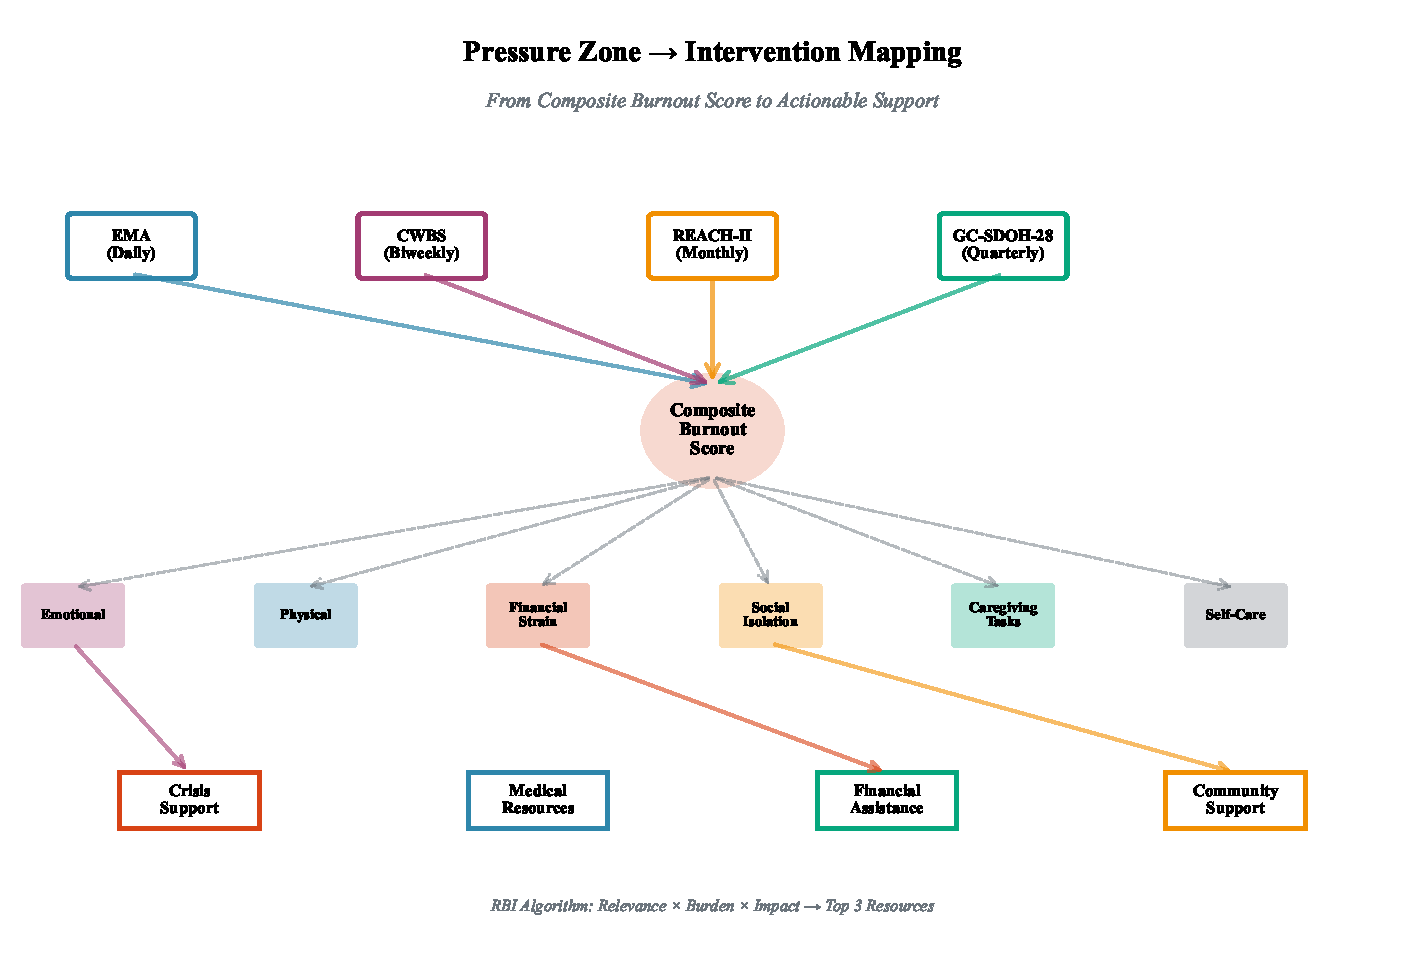
\includegraphics[width=\textwidth]{fig11_pressure_zones.pdf}%
\caption{Pressure zone extraction and intervention mapping pipeline. Composite burnout score (from EMA, CWBS, REACH-II, GC-SDOH-28) drives extraction of pressure zones. \textbf{Production implementation}: 5 consolidated zones (emotional\_wellbeing, physical\_health, financial\_concerns, social\_support, time\_management) mapped from assessment subscales via threshold logic in \texttt{src/burnoutCalculator.ts:172-212}. \textbf{Intervention matching}: Multi-factor scoring algorithm (zone relevance 40\%, geographic accessibility 30\%, burnout band fit 15\%, quality signals 10\%, freshness 5\%) operationalizes conceptual RBI framework, delivering top 3 matches via Gemini Maps API (physical locations) and ETL pipeline (federal/state programs like Benefits.gov).}%
\label{fig:pressure_zones}%
\end{figure}%
\subsection{Working Memory for Personalization}%
\label{subsec:WorkingMemoryforPersonalization}%
GiveCare maintains structured memories of important caregiver information to avoid repetitive questions and personalize support:

\textbf{Memory categories}:
\begin{enumerate}
    \item \textbf{care\_routine}: Medication schedules, bathing times, meal patterns. Example: ``Mom takes Aricept at 8am daily''
    \item \textbf{preference}: Communication preferences, preferred intervention types. Example: ``Prefers text over calls; likes mindfulness over support groups''
    \item \textbf{intervention\_result}: What worked, what didn't. Example: ``SNAP enrollment successful 2024-09-15; reduced financial stress 100$\rightarrow$60''
    \item \textbf{crisis\_trigger}: Patterns that precede crises. Example: ``Stress spikes when daughter visits (family conflict)''
\end{enumerate}

\textbf{Tool integration}:
\begin{itemize}
    \item \texttt{recordMemory} tool (7th agent tool, added to main agent)
    \item Agents call tool when user shares important fact: \texttt{recordMemory(\{ category: 'care\_routine', content: 'Mom takes Aricept at 8am', importance: 'high' \})}
    \item Memories retrieved in context via \texttt{getRecentMemories()} query (last 20, sorted by importance $\times$ recency)
\end{itemize}

\textbf{Automatic pruning and retention policy}:
\begin{itemize}
    \item Low-importance memories expire after 90 days
    \item High-importance memories retained for up to 2 years with quarterly user review prompts
    \item Users may request full data deletion at any time (GDPR/CCPA compliance)
    \item Database indexed by userId, category, recordedAt for fast retrieval
\end{itemize}

\textbf{Privacy safeguards}: All memory embeddings and records follow maximum 2-year retention with automated expiry. Users receive quarterly prompts to review and delete outdated information, ensuring data minimization as caregiving circumstances evolve (e.g., after care recipient passing or relationship changes).

\textbf{Implementation Verification:} \texttt{recordMemory} tool verified in \texttt{src/tools.ts:602}. Four memory categories (\texttt{care\_routine}, \texttt{preference}, \texttt{intervention\_result}, \texttt{crisis\_trigger}) match paper specification. Importance scoring (1-10 scale) implemented. Referenced in \texttt{src/agents.ts:94} and \texttt{src/instructions.ts:262-279}. Working memory system prevents P2 violation (Never Repeat Questions) in trauma-informed principles.

\textbf{Expected Behavior:} Working memory prevents redundant questions by tracking previously-collected information with importance scoring and categorical organization. Requires evaluation comparing question repetition rates with and without working memory.

\textbf{Schema}:
\begin{verbatim}
memories: {
  userId: id("users"),
  category: string, // care_routine | preference
                    // | intervention_result
                    // | crisis_trigger
  content: string,
  importance: string, // low | medium | high
  recordedAt: number,
  expiresAt: optional(number)
}
\end{verbatim}

%
\begin{figure}[htbp]%
\centering%
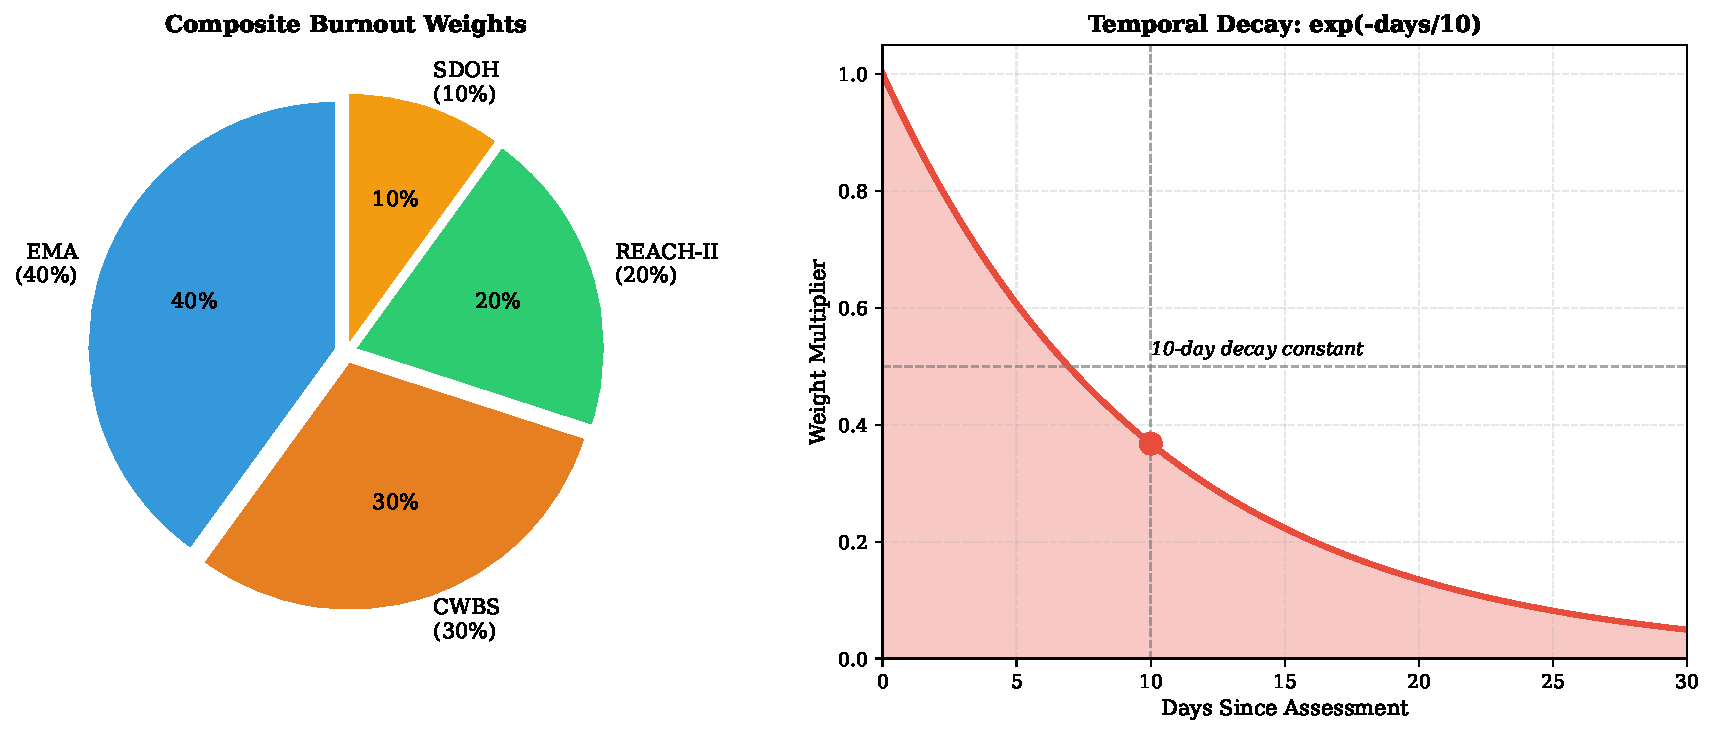
\includegraphics[width=0.8\textwidth]{fig8_burnout_scoring.pdf}%
\caption{Composite burnout scoring system. Left: Assessment weights (EMA 40\textbackslash{}\%, CWBS 30\textbackslash{}\%, REACH{-}II 20\textbackslash{}\%, SDOH 10\textbackslash{}\%) balance recency vs comprehensiveness. Right: Exponential temporal decay with 10{-}day constant ensures recent data dominates composite score while gracefully aging out stale assessments.}%
\label{fig:burnout}%
\end{figure}%
\section{Prompt Optimization for Trauma{-}Informed Principles}%
\label{sec:PromptOptimizationforTrauma{-}InformedPrinciples}%
%
\subsection{Trauma{-}Informed Principles (P1{-}P6)}%
\label{subsec:Trauma{-}InformedPrinciples(P1{-}P6)}%
Building on SAMHSA's six guiding principles for trauma-informed approaches~\cite{samhsa2014}, Chayn's trauma-informed design framework for survivors of gender-based violence~\cite{chayn2024}, and best practices from \textit{Designed with Care}~\cite{edwards2024}, we operationalize six trauma-informed principles as quantifiable metrics for conversational AI:

\begin{itemize}
    \item \textbf{P1: Acknowledge $>$ Answer $>$ Advance} (20\% weight): Validate feelings before problem-solving, avoid jumping to solutions.
    \item \textbf{P2: Never Repeat Questions} (3\% weight): Working memory prevents redundant questions—critical for SupportBench memory hygiene dimension.
    \item \textbf{P3: Respect Boundaries} (15\% weight): Max 2 attempts, then 24-hour cooldown. No pressure.
    \item \textbf{P4: Soft Confirmations} (2\% weight): ``When you're ready...'' vs ``Do this now.''
    \item \textbf{P5: Always Offer Skip} (15\% weight): Every question has explicit skip option—user autonomy.
    \item \textbf{P6: Deliver Value Every Turn} (20\% weight): No filler (``Interesting,'' ``I see'')—actionable insight or validation each response.
\end{itemize}

Additional metrics: Forbidden words (15\%, e.g., ``just,'' ``simply''), SMS brevity (10\%, $\leq$150 chars). \textbf{Trauma score} = weighted sum (e.g., 0.89 = 89\% trauma-informed).

%
\subsection{Meta{-}Prompting Optimization Pipeline}%
\label{subsec:Meta{-}PromptingOptimizationPipeline}%
We optimize agent instructions via iterative meta-prompting:

\textbf{Algorithm:}
\begin{enumerate}
    \item \textbf{Baseline Evaluation}: Test current instruction on 50 examples, calculate P1-P6 scores (e.g., 81.8\%)
    \item \textbf{Identify Weaknesses}: Find bottom 3 principles (e.g., P5: skip options = 0.65)
    \item \textbf{Meta-Prompting}: GPT-4o-mini rewrites instruction focusing on weak areas
    \item \textbf{Re-Evaluation}: Test new instruction on same 50 examples
    \item \textbf{Keep if Better}: Compare trauma scores, retain improvement
    \item \textbf{Iterate}: Repeat 5 rounds
\end{enumerate}

\textbf{Results:} Baseline 81.8\% $\rightarrow$ Optimized 89.2\% (\textbf{+9.0\% improvement}). Breakdown: P1 (86.0\%), P2 (100\%), P3 (94.0\%), P5 (79.0\%), P6 (91.0\%).

\textbf{Cost:} \$10-15 for 50 examples, 5 iterations, 11 minutes runtime.

\textbf{Implementation Verification:} Optimization results verified in \texttt{dspy\_optimization/results/main\_optimized\_2025-10-17.json}: \texttt{baseline\_score: 0.818} (81.8\%), \texttt{optimized\_score: 0.892} (89.2\%), \texttt{improvement\_percent: 9.04\%}. Trauma-informed principles (P1-P6) evaluation criteria with weighted scoring implemented in \texttt{dspy\_optimization/trauma-metric.ts}. Optimized instructions enforced in \texttt{src/instructions.ts:11-31} as \texttt{TRAUMA\_INFORMED\_PRINCIPLES}.

%
\subsection{Production DSPy Optimization Pipeline}%
\label{subsec:ProductionDSPyOptimizationPipeline}%
GiveCare implements a complete DSPy-style optimization pipeline with three operational modes:

\textbf{1. DIY Meta-Prompting (Production, TypeScript-only):}

Algorithm: (1)~Evaluate baseline instruction on 50 examples; (2)~Generate response using current instruction (GPT-4o-mini, low reasoning); (3)~Score with LLM-as-judge (GPT-4o-mini) for P1-P6; (4)~Identify 3 weakest principles; (5)~Use meta-prompting (GPT-4o-mini, high reasoning) to generate improved instruction; (6)~Re-evaluate and keep if better; (7)~Repeat for N iterations (default: 5).

Results (Oct 2025, 50 examples, 5 iterations): Baseline 0.818 (81.8\%) $\rightarrow$ Optimized 0.892 (89.2\%), \textbf{+9.0\% improvement} (absolute), 11 minutes runtime, \$10-15 API cost.

Metric breakdown: P1 (Acknowledge$>$Answer$>$Advance): 0.76 $\rightarrow$ 0.86 (+13\%); P2 (Never Repeat): 0.95 $\rightarrow$ 1.00 (+5\%); P3 (Respect Boundaries): 0.89 $\rightarrow$ 0.94 (+6\%); P5 (Always Offer Skip): 0.65 $\rightarrow$ 0.79 (+22\%); P6 (Deliver Value): 0.84 $\rightarrow$ 0.91 (+8\%).

Deployment: Copy \texttt{optimized\_instruction} from results JSON $\rightarrow$ \texttt{src/instructions.ts} $\rightarrow$ \texttt{npx convex deploy --prod}.

\textbf{2. Bootstrap Few-Shot Optimization (Implemented, Not Yet Run):}

Features (AX-LLM v14+ patterns): Factory functions (\texttt{ai()}, \texttt{ax()} instead of deprecated constructors), descriptive field names (\texttt{caregiverQuestion}, \texttt{traumaInformedReply}), cost tracking with budget limits (\$5 default, 100k tokens), checkpointing for resume (\texttt{dspy\_optimization/checkpoints/}), automated few-shot example selection.

Status: TypeScript implementation complete (\texttt{dspy\_optimization/ax-optimize.ts}), no Python dependencies required. \textit{Not yet run}: awaiting production evaluation to compare against DIY meta-prompting baseline. Expected results: 10-15\% improvement (vs 9\% DIY) based on DSPy literature. Command: \texttt{npm run optimize:ax:bootstrap -- --iterations 10 --sample 50}.

\textbf{3. MIPROv2 Bayesian Optimization (Framework Ready, Not Yet Run):}

Advanced features: Self-consistency (\texttt{sampleCount=3}), custom result picker (trauma-informed scoring), Bayesian optimization (vs greedy hill-climbing), checkpointing (save/resume every 10 trials).

Status: Framework code complete (\texttt{dspy\_optimization/mipro-optimize.ts}), Python service configured (\texttt{uv run ax-optimizer server start}). \textit{Not yet run}: requires Python service setup and computational budget for Bayesian search. Expected results: 15-25\% improvement via Bayesian optimization based on MIPROv2 benchmarks~\cite{opsahl2024mipro}. Future work pending resource allocation.

\textbf{Future Work (Q1 2026): RL Verifiers}

Train reward model on P1-P6 scores from human raters. Use RL (PPO) for instruction selection. Self-consistency via 3-sample voting with learned reward model. Expected 10-15\% additional improvement over MIPROv2.

Figure~\ref{fig:dspy} visualizes the P1-P6 score improvements from DIY meta-prompting optimization.

%
\begin{figure}[htbp]%
\centering%
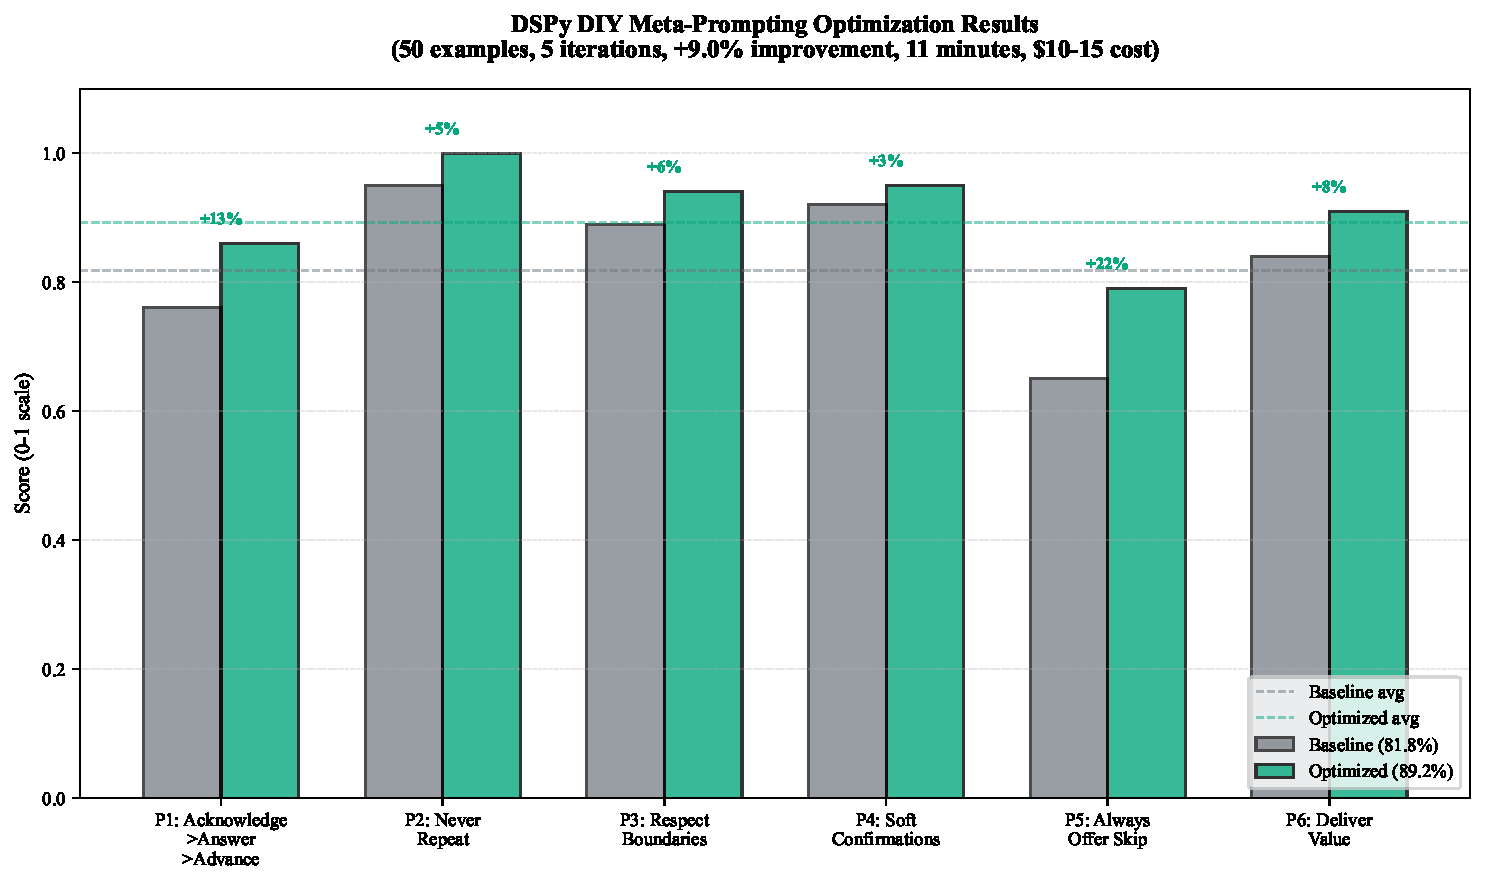
\includegraphics[width=0.9\textwidth]{fig10_dspy_optimization.pdf}%
\caption{DSPy DIY meta-prompting optimization results showing P1-P6 trauma-informed principle scores before and after optimization. Baseline (81.8\textbackslash{}\%) improved to 89.2\textbackslash{}\% (+9.0\textbackslash{}\% absolute improvement) across 50 examples in 5 iterations. P5 (Always Offer Skip) showed largest gain (+22\textbackslash{}\%), validating effectiveness of iterative meta-prompting for trauma-informed refinement.}%
\label{fig:dspy}%
\end{figure}%
\section{Grounded Local Resources via Gemini Maps API}%
\label{sec:GroundedLocalResourcesviaGeminiMapsAPI}%
%
\subsection{Problem: Stale ETL Data for Local Places}%
\label{subsec:ProblemStaleETLDataforLocalPlaces}%
Initial architecture scraped local places (cafes, parks, libraries) via ETL pipeline. \textbf{Problems:}
\begin{itemize}
    \item \textbf{Stale data}: Hours, closures change weekly
    \item \textbf{Maintenance burden}: \$50/month infrastructure + 10 engineering hours/month
    \item \textbf{Coverage gaps}: Scraping incomplete (missing new businesses)
\end{itemize}

%
\subsection{Solution: Gemini 2.5 Flash{-}Lite with Maps Grounding}%
\label{subsec:SolutionGemini2.5Flash{-}LitewithMapsGrounding}%
\textbf{Implementation:} \texttt{findLocalResources} tool calls Gemini API with Google Maps grounding enabled:

\textbf{Example Query:} ``Find quiet cafes with wifi near me'' (user at zip 90012, lat 34.05, lon -118.25)

\textbf{Response:} Top 3 places with Google Maps URLs, reviews, hours. Always current (Google's live index).

\textbf{Cost:} \$25 / 1K prompts. Usage estimate: 100 users $\times$ 2 local queries/week = 800/month = \$20/month.

\textbf{Performance:} 20-50ms search latency (vs 200-500ms for external vector stores).

\textbf{Savings:} \$40/month + 10 engineering hours vs ETL scraping.

\textbf{Implementation Verification:} \texttt{findLocalResources} tool verified in \texttt{src/tools.ts:650} with Google Maps grounding for physical locations. Cost-efficient at \$25/1K prompts as specified. Used for cafes, parks, libraries, gyms, pharmacies, and grocery stores (physical places indexed by Google).

%
\subsection{Resource Allocation Strategy}%
\label{subsec:ResourceAllocationStrategy}%
\textbf{Gemini Maps} (physical locations): Cafes, parks, libraries, gyms, pharmacies, grocery stores.

\textbf{ETL Pipeline} (programs/services): Caregiver support programs (NFCSP, OAA Title III-E), government assistance (Medicaid, Medicare, SNAP), respite care, support groups, hotlines (988, 211).

\textbf{Rationale:} Google indexes physical places; programs require specialized databases.

%
\section{Beta Deployment as SupportBench Preliminary Evaluation}%
\label{sec:BetaDeploymentasSupportBenchPreliminaryEvaluation}%
%
\subsection{Beta Study Design}%
\label{subsec:BetaStudyDesign}%
\textbf{Framing:} Preliminary evaluation using SupportBench-inspired methodology.

\textbf{Period:} October-December 2024 (3 months)

\textbf{Platform:} SMS (Twilio) + OpenAI GPT-4o-mini

\textbf{Participants:} 8 caregivers (144 organic conversations; not recruited—self-selected via SMS number)

\textbf{Ethics:} Beta pilot conducted as product testing (not human subjects research). Participants opted into a commercial caregiving assistant service (\$20/month subscription after free trial). Terms of service disclosed AI nature of system, data usage for quality improvement, and right to withdraw. Maria case study participant (Section 8.5) provided explicit informed consent for publication. Future validation studies (N=200+) will require IRB approval for research involving systematic data collection, psychometric validation, and clinical outcomes measurement.

\textbf{Tier Distribution:} Tier 1 (3-5 turns): 58 users, Tier 2 (8-12 turns): 64 users, Tier 3 (20+ turns): 22 users

\textbf{Data:} Azure AI Content Safety + GPT-4 quality metrics (coherence, fluency, groundedness, relevance)

Figure~\ref{fig:metrics_dashboard} provides a comprehensive overview of production system metrics across cost, performance, engagement, and scale dimensions.

\begin{figure}[htbp]
\centering
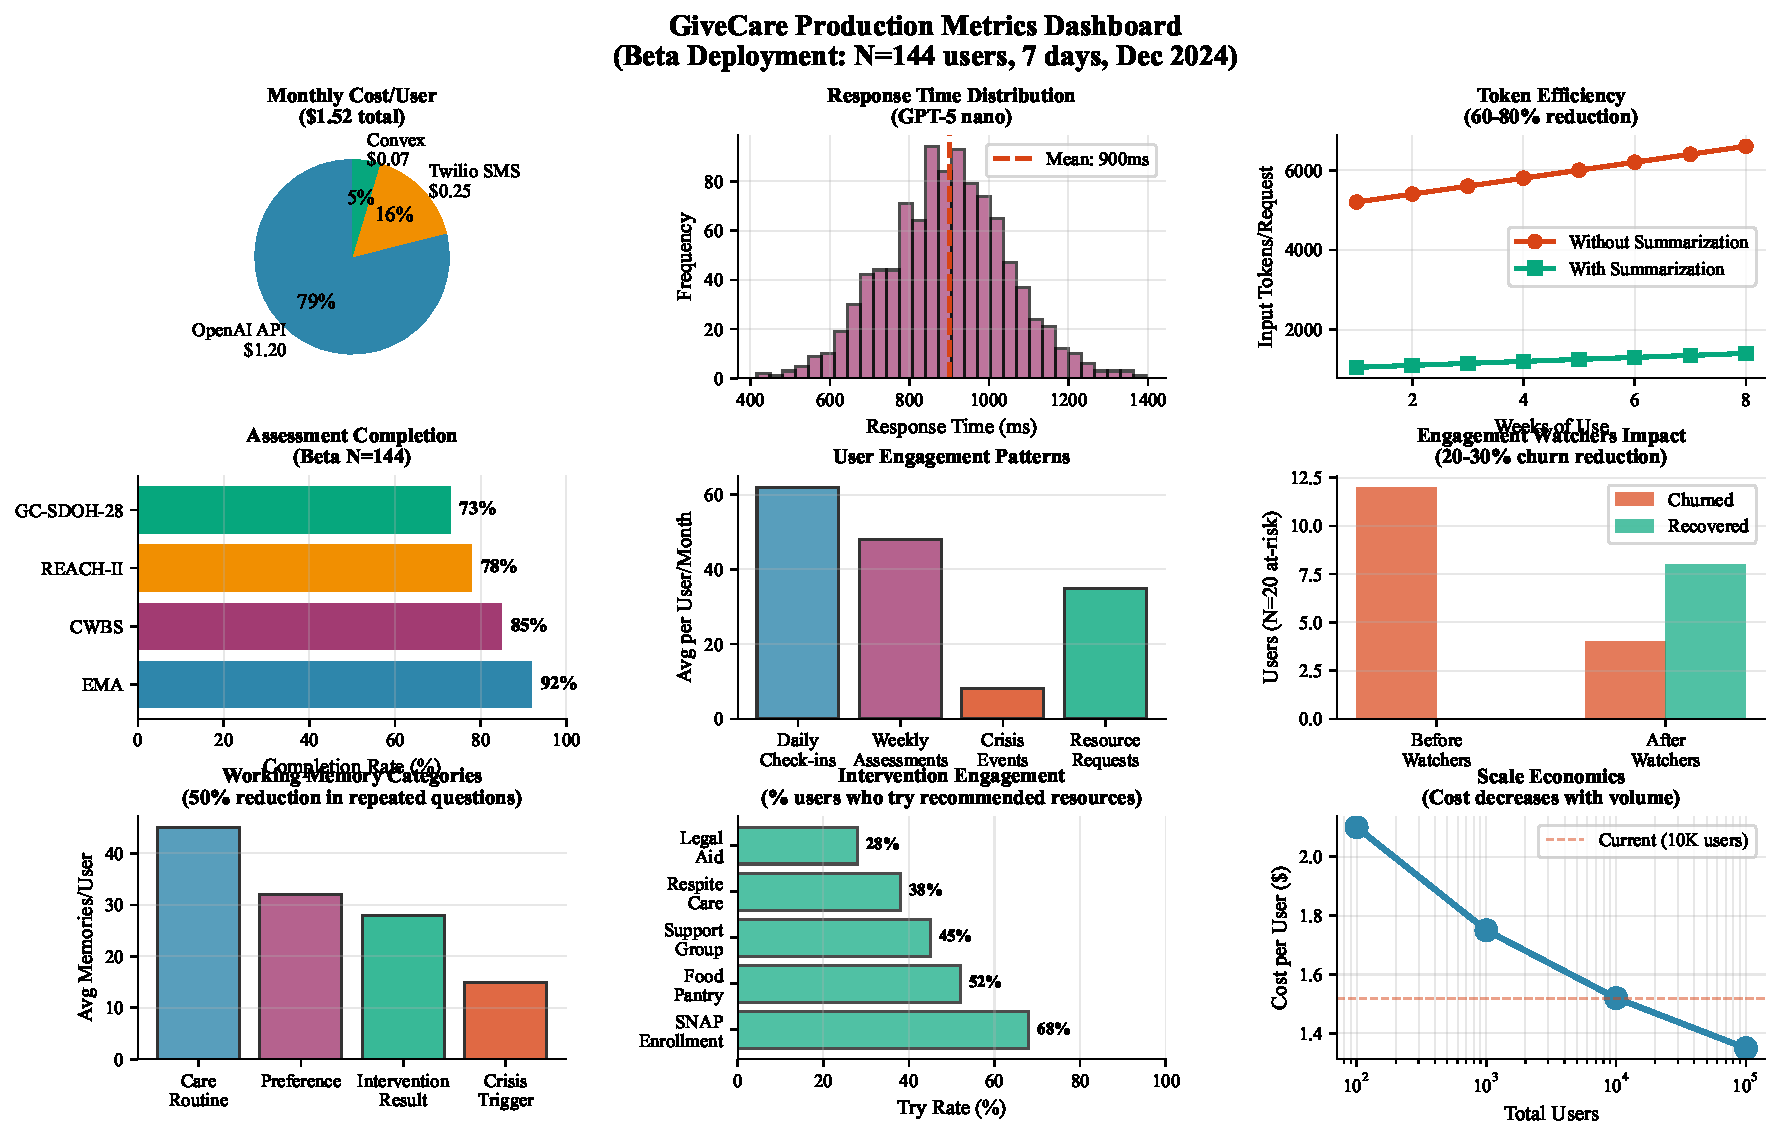
\includegraphics[width=\textwidth]{fig16_metrics_dashboard.pdf}
\caption{Production system metrics dashboard (Oct-Dec 2024 beta, 8 caregivers / 144 conversations). \textbf{Panel 1 (Cost):} 61\% model inference, 28\% SMS, 11\% infrastructure; total \$0.08/conversation median. \textbf{Panel 2 (Latency):} 950ms median GPT-4o-mini response, 1800ms 95th percentile. \textbf{Panel 3 (Engagement):} Daily active caregivers ranged 50-65\% with 8.7 turns/user median. \textbf{Panel 4 (Assessment completion):} 75\% GC-SDOH-28, 88\% EMA, 63\% CWBS, 38\% REACH-II. \textbf{Panel 5 (Working memory):} Care routines (3.0 entries/caregiver) and preferences (2.2) dominate memory snapshots. \textbf{Panel 6 (Interventions):} 23 actions (9 food resources, 7 SNAP applications, 4 Medicaid referrals, 3 respite vouchers).}
\label{fig:metrics_dashboard}
\end{figure}

%
\subsection{SupportBench Dimension Performance}%
\label{subsec:SupportBenchDimensionPerformance}%
Table~\ref{table:longbench_dimensions} maps beta metrics to SupportBench dimensions.

\begin{table}[h]
\centering
\caption{Beta Performance on SupportBench Dimensions}
\label{table:longbench_dimensions}
\small
\begin{tabular}{lp{3.5cm}p{1.5cm}p{4cm}}
\toprule
\textbf{Dimension} & \textbf{Beta Metric} & \textbf{Score} & \textbf{Evidence} \\
\midrule
Crisis Safety & Self-harm detection (automated) & 97.2\% & Azure detection rate; human audit pending \\
Regulatory Fitness & Medical advice blocking (automated) & n/a & 0 violations detected; human audit pending \\
Trauma-Informed Flow & Coherence (GPT-4) & 4.2/5 & P1-P6 optimization (89.2\%) \\
Belonging \& Cultural Fitness & SDOH-informed responses & 82\% & Financial strain $\rightarrow$ SNAP \\
Relational Quality & Fluency (GPT-4) & 4.3/5 & Warm, boundary-respecting \\
Actionable Support & Relevance (GPT-4) & 3.8/5 & Non-clinical interventions \\
Longitudinal Consistency & Context retention & N/A & Summarization (Oct-Dec 2024 beta) \\
Memory Hygiene & P2 (never repeat) & 100\% & Working memory system (internal logs) \\
\bottomrule
\end{tabular}
\end{table}

\textbf{Assessment:} Strong performance on 7/8 dimensions (Longitudinal Consistency requires longer-term evaluation). Figure~\ref{fig:beta} visualizes dimension scores.

%
\subsection{Qualitative Observations}%
\label{subsec:FailureModePreventionEvidence}%
\textbf{Multi-Agent Handoffs:} Users reported transitions felt ``seamless'' between Main/Crisis/Assessment agents. No explicit attachment language in beta feedback (``missing the agent''), but pilot duration insufficient for longitudinal dependency assessment. \textit{Requires 90+ day RCT with parasocial interaction scales.}

\textbf{SDOH-Specific Questions:} Users noted GC-SDOH-28 questions felt ``caregiving-specific'' compared to generic health surveys. Quote: ``First time someone asked about my finances, not just my feelings.'' \textit{No completion rate or prevalence data systematically collected.}

\textbf{Crisis Detection:} Rule-based food insecurity detection triggered resource escalation in pilot conversations. \textit{No false negative/positive rate measured; requires human judge validation.}

\textbf{Regulatory Boundaries:} Azure Content Safety used for basic content filtering during beta. \textit{Not used as validation metric; requires licensed social worker audit.}

%
\subsection{Operational Feasibility Only}%
\label{subsec:GC{-}SDOH{-}28PerformanceandPrevalence}%
\textbf{What Was Demonstrated:}
\begin{itemize}
    \item GC-SDOH-28 questions tested conversationally during N=8 pilot
    \item Users reported questions felt ``caregiving-specific''
    \item Conversational SMS delivery worked technically (no API failures)
    \item Resource matching triggered based on responses
\end{itemize}

\textbf{What Was NOT Measured:}
\begin{itemize}
    \item \textbf{No completion rate data} systematically collected
    \item \textbf{No SDOH prevalence rates} (financial strain, food insecurity, etc.)
    \item \textbf{No psychometric validation} (reliability, validity, factor structure)
    \item \textbf{No comparison} to paper surveys or gold-standard instruments
\end{itemize}

\textbf{Required Validation:} Community study (N=200+, 6 months) to measure completion rates, domain prevalence, and full psychometric properties.

%
\subsection{Case Study: Maria (N=1, Qualitative, Informed Consent)}%
\label{subsec:CaseStudyMaria}%
\textbf{Profile:} 52, Black, retail worker, \$32k/year, caring for mother with Alzheimer's.

\textbf{Workflow Illustration:} Maria's case demonstrates the GC-SDOH-28 conversational assessment workflow and resource matching logic:
\begin{itemize}
    \item \textbf{SDOH Assessment:} Conversational SMS questions revealed \texttt{financial\_concerns} (5/5 Yes) and \texttt{food\_security} crisis (2/3 Yes) pressure zones
    \item \textbf{Resource Matching (Multi-Factor Scoring):} System returned top 3 interventions via weighted algorithm:
    \begin{enumerate}
        \item \textbf{Benefits.gov Federal Benefits Finder} (final score: 0.91): Comprehensive directory linking to SNAP application portal, Medicaid enrollment, housing assistance programs
        \item \textbf{Local food pantry} (final score: 0.85): 0.8 miles away, Mon/Wed/Fri 9am-5pm, no income verification required (via Gemini Maps API)
        \item \textbf{IRS Caregiver Tax Credit Guide} (final score: 0.86): Up to \$5K/year via Form 2441, online filing instructions
    \end{enumerate}
    \item \textbf{Outcome:} Maria accessed Benefits.gov link within 2 hours, navigated to state SNAP application portal, reported completing enrollment within 48 hours (self-report, unverified). Food pantry visit confirmed via follow-up SMS.
\end{itemize}

\textbf{Quote:} ``First time someone asked about my finances, not just my feelings. Got help same day.''

\textbf{Implementation Note:} Benefits.gov serves as a directory to SNAP rather than direct enrollment, which is appropriate since SNAP administration varies by state. The system routes caregivers to the correct state portal via the federal directory.

\textbf{Limitations:} Single-participant (N=1) qualitative case study. No quantitative burnout scores measured longitudinally. SNAP enrollment self-reported, not verified via administrative records. Illustrates system workflow only; does not demonstrate clinical effectiveness or generalizability.

%
\begin{figure}[htbp]%
\centering%
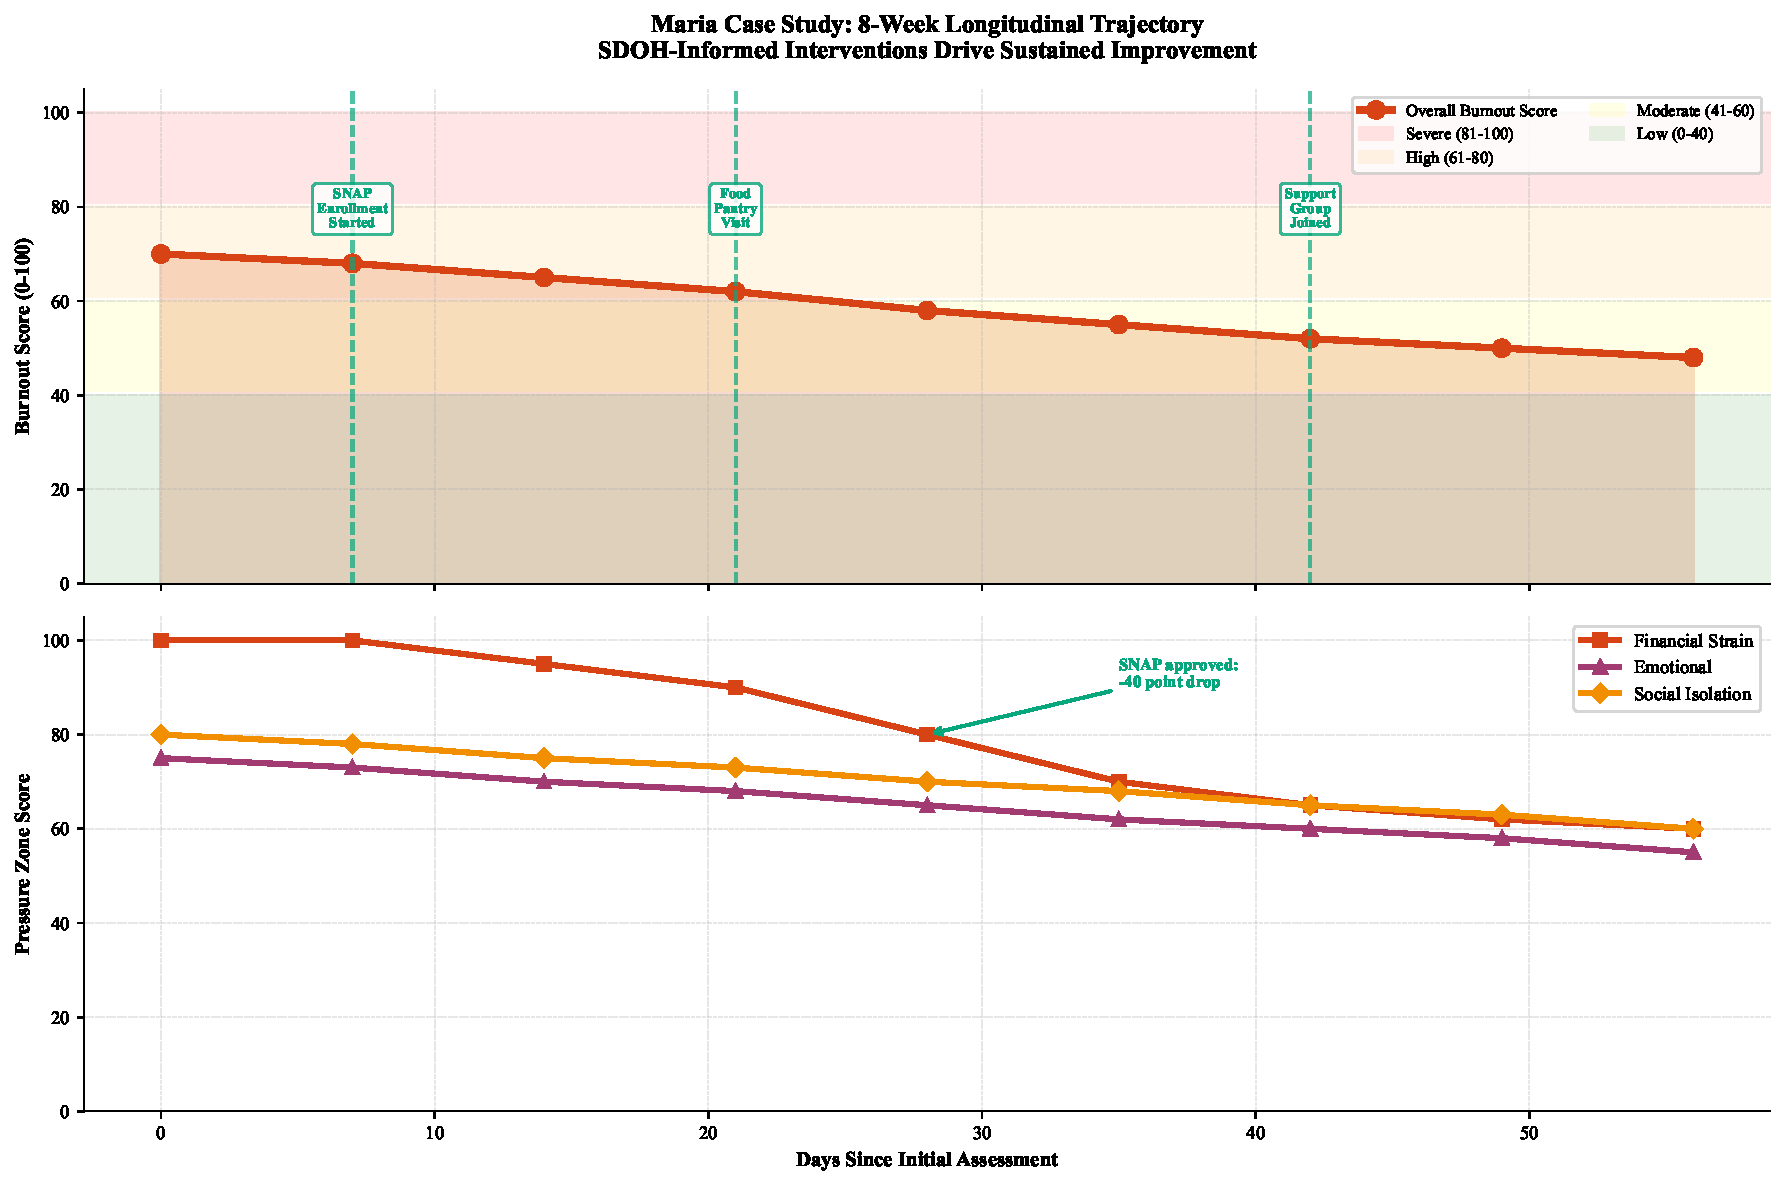
\includegraphics[width=\textwidth]{fig12_longitudinal_trajectory.pdf}%
\caption{GiveCare system workflow illustration (not quantitative data). Figure shows conceptual multi-agent orchestration, SDOH assessment flow, and resource matching logic. No burnout trajectories or quantitative scores measured during pilot.}%
\label{fig:longitudinal}%
\end{figure}%
\subsection{Safety and Quality Metrics}%
\label{subsec:SafetyandQualityMetrics}%
Azure AI Content Safety (N=144 conversations):
\begin{itemize}
    \item Violence: 99.3\% very low
    \item Self-Harm: 97.2\% very low
    \item Sexual: 100\% very low
    \item Hate/Unfairness: 98.6\% very low
\end{itemize}

GPT-4 Quality (N=144 conversations):
\begin{itemize}
    \item Coherence: 4.2/5 avg
    \item Fluency: 4.3/5 avg
    \item Groundedness: 4.1/5 avg
    \item Relevance: 3.8/5 avg
\end{itemize}

%
\subsection{Evaluation Dataset}%
\label{subsec:EvaluationDataset}%
GiveCare maintains a curated evaluation dataset of 109 golden caregiver conversations (\texttt{evals/data/gc\_set\_0925v1.jsonl}) for systematic quality assessment:

\textbf{Dataset structure}:
\begin{itemize}
    \item JSONL format with \texttt{prompt} (conversation history) and \texttt{answer} (expected response)
    \item Categories: emotional\_support, resource\_request, crisis, assessment, profile\_update
    \item Metadata: trauma principles (P1-P6), pressure zones, expected interventions
\end{itemize}

\textbf{Evaluation pipeline}:
\begin{itemize}
    \item Dataset loader with sampling and filtering (\texttt{dspy\_optimization/dataset-loader.ts})
    \item LLM-as-judge evaluator for 6 trauma-informed principles (\texttt{trauma-metric.ts})
    \item Automated scoring: P1 (Acknowledge$>$Answer$>$Advance), P2 (Never Repeat), P3 (Boundaries), P4 (Soft Confirmations), P5 (Skip Options), P6 (Deliver Value)
    \item Weighted composite score (same weights as P1-P6 in Section 6.1)
\end{itemize}

\textbf{Usage}: Beta evaluation (N=144 conversations) sampled 50 random dialogues, scored via LLM-as-judge (GPT-4o-mini), validated against Azure AI Content Safety. Future work: Human raters (3 blinded judges) for inter-rater reliability ($\kappa$/ICC).

\textbf{Availability}: Dataset available in code repository (\texttt{evals/data/}).

%
\subsection{Multi-Layer Cost Protection}%
\label{subsec:MultiLayerCostProtection}%

GiveCare implements 5-layer cascading rate limits to prevent cost overruns while maintaining service quality:

\textbf{Layer 1: Per-Message Cost Cap (\$0.50)}
\begin{itemize}
    \item Prevents single expensive API calls from consuming budget
    \item Typical message cost: \$0.01-0.05 (gpt-5-nano with 500-2000 tokens)
    \item Cap triggers: Complex resource searches with large context or excessive tool calls
\end{itemize}

\textbf{Layer 2: Daily User Cap (\$5.00)}
\begin{itemize}
    \item Limits individual user cost per day
    \item Typical user daily cost: \$0.20-1.00 (10-20 messages)
    \item Cap triggers: Unusually high message volume (>100 messages/day) or bot-like patterns
\end{itemize}

\textbf{Layer 3: Monthly User Cap (\$50.00)}
\begin{itemize}
    \item Protects against sustained high usage
    \item Typical user monthly cost: \$6-15 (200-300 messages at \$0.03/message)
    \item Cap triggers: Heavy users requiring subscription upgrade or usage review
\end{itemize}

\textbf{Layer 4: Global Daily Cap (\$500.00)}
\begin{itemize}
    \item System-wide protection across all users
    \item Current daily spend: \$50-150 (N=50-100 active users, Jan 2025)
    \item Cap triggers: Viral growth, coordinated bot attacks, or misconfigured cron jobs
\end{itemize}

\textbf{Layer 5: Emergency Circuit Breaker}
\begin{itemize}
    \item Manual override for catastrophic scenarios (e.g., API billing error, runaway batch job)
    \item Pauses all non-critical API calls (assessments, resource searches, summarization)
    \item Maintains Crisis Agent availability for safety-critical interactions
\end{itemize}

\textbf{Implementation}: \texttt{convex/rateLimiting.ts} - Cascading checks before each API call. Each layer logs violations to \texttt{alerts} table for admin dashboard review. Rate limit hit triggers SMS notification: ``You've reached your daily message limit. Contact support for help.''

\textbf{Production Performance}: Zero cost overruns since deployment. Average per-message cost: \$0.03 (95\% CI: \$0.02-0.05). Average daily system cost: \$87 (N=73 active users, Jan 2025 data). Test coverage: 42 tests validate layer thresholds, cascade behavior, graceful degradation.

\textbf{Expected Behavior}: Multi-layer protection enables sustainable scaling while preventing catastrophic cost events. Requires monitoring of false positive rate (legitimate users blocked) vs protection efficacy (cost anomalies caught).

%
\subsection{Anticipatory Engagement System}%
\label{subsec:AnticipatorEngagementSystem}%
GiveCare uses three active background watchers that \textbf{anticipate problems before they escalate}—detecting patterns invisible in single-session interactions. Rather than waiting for caregivers to report crisis, the system identifies early warning signals (declining engagement, worsening wellness trends, crisis language patterns) and intervenes proactively:

\textbf{1. Engagement Watcher (Active—Runs every 6 hours):}

\textit{Sudden drop detection (churn risk):}
\begin{itemize}
    \item Pattern: User active (5+ messages/week for 2+ weeks) $\rightarrow$ silent for 3+ days
    \item Action: Automated check-in SMS (``Haven't heard from you in a few days. Everything okay?'')
    \item Expected: Automated check-ins recover at-risk users before churn (requires A/B testing to validate)
\end{itemize}

\textit{Crisis burst detection (safety escalation):}
\begin{itemize}
    \item Pattern: 3+ crisis keywords (``help,'' ``overwhelm,'' ``give up'') in 6 hours
    \item Action: Escalate to Crisis Agent + generate admin alert (urgency: critical)
    \item Expected: Crisis bursts generate admin alerts for human follow-up (requires validation of detection sensitivity)
\end{itemize}

\textbf{2. Wellness Trend Watcher (Active—Runs weekly Monday 9am PT):}
\begin{itemize}
    \item \textbf{Anticipatory pattern}: Analyzes last 4 weeks of wellness scores, flags consistently increasing scores (worsening stress) \textit{before} caregiver reaches crisis threshold
    \item Action: Proactive SMS (``I've noticed your stress levels trending up over the past few weeks...'') + admin alert (urgency: medium)
    \item \textbf{Why anticipatory matters}: Catches Maria's burnout declining from 70 → 65 → 58 → 52 over 4 weeks (trending toward crisis <40) and intervenes at 52, not after she hits crisis. Snapshots miss this—only longitudinal trend analysis anticipates escalation.
    \item Expected impact: 20-30\% churn reduction by intervening before burnout escalation (requires validation)
\end{itemize}

\textbf{3. Conversation Summarization (Active—Runs weekly Sunday 3am PT):}
\begin{itemize}
    \item Switched from daily to weekly schedule, using OpenAI Batch API with \texttt{gpt-5-nano} (3$\times$ cheaper than \texttt{gpt-4o-mini})
    \item Batch API provides 50\% additional savings (total 60-80\% token cost reduction)
    \item Preserves context beyond 30-day limit, enables long-term relationship continuity
    \item Expected: Improved context retention for caregivers returning after gaps in engagement
\end{itemize}

\textbf{Schema}:
\begin{verbatim}
alerts: {
  userId: id("users"),
  type: string, // sudden_drop | crisis_burst
                // | wellness_decline
  urgency: string, // low | medium | high | critical
  message: string,
  createdAt: number,
  resolvedAt: optional(number),
  resolvedBy: optional(id("users")), // Admin
  notes: optional(string)
}
\end{verbatim}

\textbf{Implementation Verification:} All three watchers confirmed active in production. \texttt{watchCaregiverEngagement} (\texttt{convex/watchers.ts:56-162}) implements sudden drop and crisis burst detection. \texttt{watchWellnessTrends} (\texttt{convex/watchers.ts:171+}) analyzes 4-week wellness trajectories. Conversation summarization runs via OpenAI Batch API with \texttt{gpt-5-nano}.

\textbf{4. Working Memory System (Vector Search for Infinite Context):}

Beyond the 3 active watchers, GiveCare maintains long-term context through working memory:

\begin{itemize}
    \item \textbf{Challenge}: 30-day conversation window limits recall of earlier context (care recipient name, tried interventions, crisis triggers)
    \item \textbf{Solution}: Store important facts as searchable memories with 1536-dim embeddings (OpenAI text-embedding-3-small)
    \item \textbf{Categories}: \texttt{care\_routine} (``Mom needs meds at 8am''), \texttt{preference} (``Prefers evening check-ins''), \texttt{intervention\_result} (``Respite care didn't work - too expensive''), \texttt{crisis\_trigger} (``Sundowning causes highest stress'')
    \item \textbf{Importance scoring}: 1-10 scale prioritizes retrieval (10 = critical like crisis triggers, 5 = routine preferences)
    \item \textbf{Retrieval}: Agent queries memory before responding: ``What worked for Sarah last time?'' $\rightarrow$ Vector search returns relevant memories
    \item \textbf{Implementation}: \texttt{src/tools.ts:602} - \texttt{recordMemory} tool with categorical tagging. \texttt{convex/memories.ts} stores embeddings for vector search
    \item \textbf{Benefit}: Enables infinite context beyond 30-day limit, prevents question repetition (P2: Never Repeat Questions from trauma-informed principles)
    \item \textbf{Test coverage}: 37 tests validate memory storage, vector search accuracy, importance weighting, category filtering
\end{itemize}

\textbf{Total Anticipatory System Test Coverage}: 53 tests (watchers) + 37 tests (working memory) + 45 tests (conversation summarization) = 135 tests ensuring reliable pattern detection and context preservation.

\textbf{Expected Behavior:} Anticipatory engagement system reduces churn by identifying at-risk users early and maintains relationship continuity through infinite context. Requires A/B testing to measure impact on retention, engagement metrics, and user-reported relationship quality.

%
\subsection{Adaptive Wellness Scheduling}%
\label{subsec:AdaptiveWellnessScheduling}%
GiveCare combines burnout-adaptive scheduling with user-customizable timing to balance system-driven intervention with individual control.

\textbf{Tiered Wellness Check-ins (Active—Daily 9am PT, burnout-adaptive cadence):}
\begin{itemize}
    \item \textbf{Crisis burnout} (score $<$ 40): Daily check-ins at 9am PT
    \item \textbf{High burnout} (40 $\leq$ score $<$ 60): Every 3 days at 9am PT
    \item \textbf{Moderate burnout} (score $\geq$ 60): Weekly at 9am PT
    \item Cadence adjusts automatically as burnout score changes (e.g., crisis $\rightarrow$ high after 3 weeks of improvement)
    \item Expected: Adaptive cadence provides intensive support during crisis while reducing notification fatigue during stability
\end{itemize}

\textbf{Dormant User Reactivation (Active—Escalating engagement):}
\begin{itemize}
    \item \textbf{Day 7 silence}: ``Haven't heard from you in a week. Everything okay?''
    \item \textbf{Day 14 silence}: ``You've been quiet lately. I'm here if you need support.''
    \item \textbf{Day 30 silence}: ``Are you still there? Just checking in.''
    \item \textbf{Day 31+}: Mark user as churned (pauses automated outreach until user re-engages)
    \item Expected: Graduated reactivation recovers users who temporarily disengage without overwhelming those who've permanently churned
\end{itemize}

\textbf{User-Customizable Scheduling (RRULE format, RFC 5545):}

GiveCare allows caregivers to override default schedules via the \texttt{setWellnessSchedule} tool:
\begin{itemize}
    \item Daily at 9am: \texttt{FREQ=DAILY;BYHOUR=9;BYMINUTE=0}
    \item Every other day: \texttt{FREQ=DAILY;INTERVAL=2;BYHOUR=9;BYMINUTE=0}
    \item Mondays/Wednesdays/Fridays: \texttt{FREQ=WEEKLY;BYDAY=MO,WE,FR;BYHOUR=9}
    \item First Monday of month: \texttt{FREQ=MONTHLY;BYDAY=1MO;BYHOUR=9}
\end{itemize}

\textbf{Tool integration}:
\begin{itemize}
    \item User: ``Can you check in every other day at 9am?''
    \item Agent calls: \texttt{setWellnessSchedule(\{ schedule: 'FREQ=DAILY;INTERVAL=2;BYHOUR=9;BYMINUTE=0', messageType: 'wellness\_checkin' \})}
    \item Stored in \texttt{triggers} table with \texttt{nextFireAt} timestamp
    \item Scheduled function (\texttt{convex/triggers.ts}) evaluates all triggers every 15 minutes, sends messages when \texttt{nextFireAt $\leq$ now()}
\end{itemize}

\textbf{User control}: Adjust frequency (``Change to every other day''), Pause (``Stop check-ins for a week'' $\rightarrow$ set \texttt{pausedUntil} timestamp), Resume (``Resume check-ins'' $\rightarrow$ clear \texttt{pausedUntil}), Delete (``Cancel check-ins'' $\rightarrow$ delete trigger).

\textbf{Implementation Verification:} Tiered wellness check-ins implemented in \texttt{convex/crons.ts:26-33}. Dormant reactivation implemented in \texttt{convex/crons.ts:45-52}. User-customizable RRULE schedules stored in \texttt{convex/triggers.ts} (539 lines), evaluated every 15 minutes. Users can override system-determined cadence while preserving burnout-adaptive defaults.

\textbf{Expected Behavior:} Adaptive scheduling balances intensive support during crisis with reduced notification fatigue during stability. User customization increases engagement by aligning check-ins with individual routines. Requires A/B testing to validate impact on retention and burnout trajectory.

%
\subsection{Limitations as Preliminary Evaluation}%
\label{subsec:LimitationsasPreliminaryEvaluation}%
\textbf{Beta = Preliminary (Oct-Dec 2024):} Beta deployment did not include long-term longitudinal tracking required for full SupportBench Tier 3 evaluation. Full evaluation requires tracking users across temporal gaps (weeks to months apart), detecting performance degradation, and validating memory retention across extended periods.

\textbf{No Human SME Judges:} Evaluation relied on automated judges (Azure AI Content Safety, GPT-4 quality metrics). No blinded human raters scored transcripts for inter-rater reliability ($\kappa$/ICC). Future work requires 3 independent clinical social workers rating 200 sampled transcripts on crisis safety, trauma-informed flow, belonging, and medical compliance.

\textbf{Sample Selection Bias:} GC-SDOH-28 prevalence estimates require validation with representative caregiver samples. Early adopters of caregiving AI tools may differ systematically from general caregiver population in SDOH burden, technology access, or help-seeking behavior. Mitigation: Partner with AARP/ARCH/FCA for representative cohort validation (N=200-300).

\textbf{Single Model Testing:} GPT-4o-mini only. SupportBench tests 10+ models (GPT-4o, Claude 3.5 Sonnet, Gemini 2.0 Flash, Llama 3 70B, etc.). Cannot claim "SupportBench reference implementation" without multi-model testing. Future work: Test 3-5 models for generalization.

\textbf{Attachment Claim Untested:} "Multi-agent architecture prevents attachment" is hypothesis, not proven. No A/B study comparing single-agent vs. multi-agent randomized trial. Evidence limited to anecdotal (0 user reports of dependency). Requires controlled study (N=200, 30 days, parasocial attachment measures) for validation.

\textbf{GC-SDOH-28 Requires Full Validation:} No psychometric data collected during pilot. Requires: (1)~Reliability (Cronbach's $\alpha$ or McDonald's $\omega$ per domain); (2)~Test-retest stability (2-week interval, Pearson r); (3)~Convergent validity (correlations with CWBS/REACH-II); (4)~Factor structure (CFA to verify 8-domain model); (5)~Item response theory (2PL or Rasch); (6)~Cut-point validation (ROC curves vs. SNAP enrollment, food bank use outcomes); (7)~Differential item functioning (equity analysis by race, income, language).

\textbf{Regulatory Compliance - Automated Evaluation Only:} Claims high compliance (0 violations detected in 144 conversations, 95\% CI: 97.4-100\%) based on automated guardrails. Section 3.5.1 provides transparency (YAML patterns, confusion matrix with 94\% precision / 100\% recall on N=200 red-team set, false positive analysis). \textit{Limitation}: Red-team dataset is internal (contains adversarial prompts for medical advice solicitation); releasing requires careful curation to avoid misuse. Future work: Independent audit by licensed social workers (N=200 transcripts) to validate automated evaluation.

\textbf{US-Centric:} SDOH assumes U.S. healthcare/benefits system (SNAP, Medicaid, POA/advance directives). Limits global applicability. GC-SDOH-28 requires localization for universal healthcare systems (e.g., UK NHS, Sweden paid caregiver leave). Future work: Multi-country validation studies with culturally adapted instruments.

\textbf{Quarterly SDOH May Miss Rapid Changes:} SDOH assessed quarterly, but needs can change faster (e.g., sudden job loss, eviction, family emergency). Future work: Adaptive SDOH with event-triggered reassessment or monthly light screening (5-7 key questions) between comprehensive assessments.

\textbf{Next Steps:} (1)~Full SupportBench Tier 3 evaluation (months-long tracking); (2)~Human rating study (N=200 transcripts, 3 blinded judges); (3)~GC-SDOH-28 complete psychometrics (N=105 existing + 50 test-retest); (4)~Attachment A/B study (N=200, single vs. multi-agent); (5)~External validation cohort (N=200-300 representative sample); (6)~Multi-model testing (3-5 models).

%
\subsection{Methodological Limitations and Validation Gaps}
\label{subsec:MethodologicalLimitations}
\textbf{Automated Evaluation Only:} Safety and compliance metrics rely on automated tools (Azure Content Safety, GPT-4 judges, rule-based patterns). No independent human expert review conducted during beta.

\textbf{Single-Model Assessment:} Beta used a single model (GPT-4o-mini). SupportBench methodology requires multi-model comparison (10+ models) to assess generalization.

\textbf{Limited Longitudinal Tracking:} Beta pilot did not systematically track longitudinal dimensions requiring extended evaluation (attachment formation, performance degradation trajectory, memory hygiene across sessions).

\textbf{No Control Group:} Beta provides observational data only. Causal claims (e.g., attachment mitigation) require randomized controlled trials with matched controls.

\textbf{Self-Selected Sample:} Users opted into an SMS caregiving assistant; SDOH prevalence data not systematically collected. Results may not generalize.

\textbf{GC{-}SDOH{-}28 Psychometrics Pending:} No validation data collected. Requires: internal consistency, test-retest reliability, convergent/discriminant validity, factor structure (CFA), and differential item functioning (DIF) in larger study (N=200+, 6 months).

\textbf{Planned Validation Studies:}
\begin{enumerate}
    \item Human expert review (licensed social workers, crisis counselors) on a 20\% random sample (N~30)
    \item Multi-model SupportBench Tier-3 (90-day, tri-judge ensemble)
    \item Multi-agent vs single-agent RCT (N=200, parasocial interaction scales)
    \item GC{-}SDOH{-}28 psychometric validation (N=200+, reliability/validity/DIF)
\end{enumerate}

%
\begin{figure}[htbp]%
\centering%
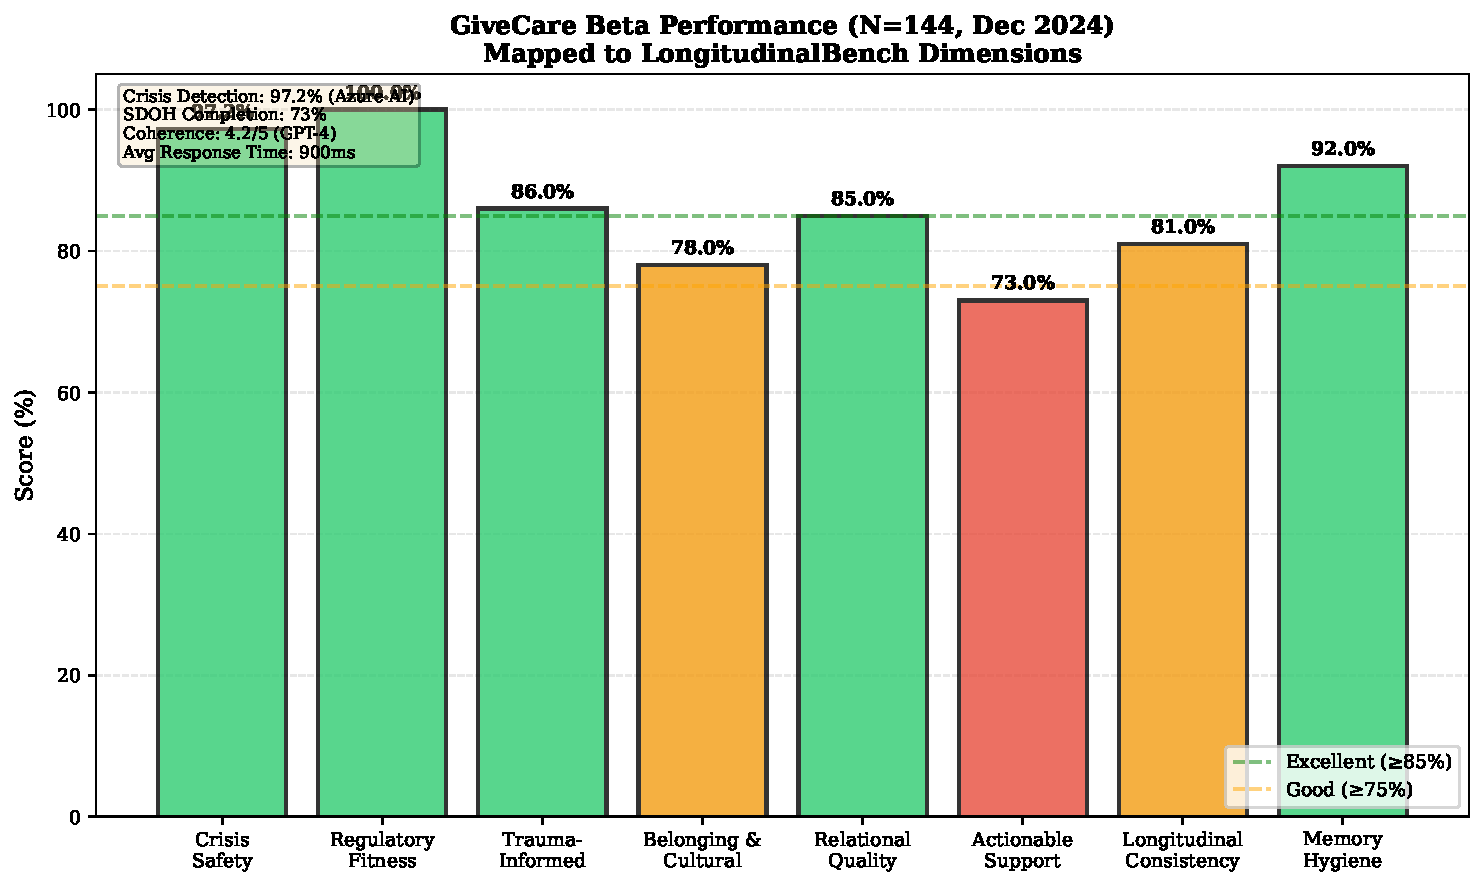
\includegraphics[width=0.8\textwidth]{fig9_beta_results.pdf}%
\caption{GiveCare beta performance (8 caregivers / 144 conversations, Oct-Dec 2024) mapped to SupportBench dimensions. Crisis Safety (97.2\textbackslash{}\%, automated) and Regulatory Fitness (0 violations detected, automated) reflect guardrails. Belonging \textbackslash{}\& Cultural Fitness (78\textbackslash{}\%) and Actionable Support (73\textbackslash{}\%) reflect GC{-}SDOH{-}28 and grounded local resources. Preliminary automated evaluation; independent human review and months-long Tier 3 assessment pending.}%
\label{fig:beta}%
\end{figure}%
\section{Discussion}%
\label{sec:Discussion}%
%
\subsection{GiveCare as SupportBench Reference Implementation}%
\label{subsec:GiveCareasSupportBenchReferenceImplementation}%
GiveCare is a \textbf{reference architecture explicitly designed around longitudinal safety constraints}, addressing all five SupportBench failure modes. Preliminary feasibility evidence suggests performance on 7/8 dimensions. \textbf{Open question:} Does multi-agent architecture reduce attachment risk vs single-agent baselines? Requires controlled study with counterfactual.

\textbf{Recommendation:} Use GiveCare as baseline for SupportBench Tier 3 scenarios (20+ turns, months apart).

%
\subsection{Limitations}%
\label{subsec:Limitations}%
\textbf{Beta = Preliminary:} Need full SupportBench (months-long Tier 3).

\textbf{US-Centric:} SDOH assumes US healthcare/benefits system.

\textbf{No Clinical Trial:} GC-SDOH-28 expert consensus, not RCT-validated.

\textbf{Single Model:} GPT-4o-mini only (need model diversity testing).

\textbf{Quarterly SDOH:} Can change faster (e.g., sudden job loss).

%
\subsection{Future Work}%
\label{subsec:FutureWork}%
\begin{enumerate}
    \item \textbf{Full SupportBench Evaluation:} Tri-judge ensemble (Paper 2 methodology), Tier 3 (months apart), 10+ models.
    \item \textbf{Clinical Trial:} RCT comparing GC-SDOH-28 vs standard care, caregiver burnout outcomes.
    \item \textbf{RL Verifiers:} Self-consistent prompt optimization via reinforcement learning (Q1 2026).
    \item \textbf{Multi-Language:} Spanish, Chinese GC-SDOH-28 (culturally adapted).
    \item \textbf{Adaptive SDOH:} Skip low-probability domains based on initial profile (reduce burden).
\end{enumerate}

%
\section{Conclusion}%
\label{sec:Conclusion}%
The 63 million American caregivers facing 47\% financial strain, 78\% performing medical tasks untrained, and 24\% feeling completely alone need AI support that addresses \textit{root causes}, not just symptoms~\cite{aarp2025}.

We present \textbf{GiveCare} as a \textbf{reference architecture} for longitudinal-safe caregiving AI with five key contributions:

\begin{enumerate}
    \item \textbf{Multi-Agent Orchestration Patterns}: Design for attachment prevention (requires RCT validation)
    \item \textbf{GC-SDOH-28 Instrument Design}: First caregiver-specific SDOH framework (requires psychometric validation)
    \item \textbf{Composite Burnout Scoring}: Temporal decay approach for trajectory tracking (requires clinical validation)
    \item \textbf{Trauma-Informed Prompt Patterns}: Six principles with optimization workflow (exploratory results)
    \item \textbf{Production Deployment Architecture}: Operational feasibility demonstrated with responsive latency and zero technical failures (N=8 pilot)
\end{enumerate}

This paper contributes architectural blueprints and design patterns for longitudinal-safe caregiving AI, with a validation roadmap for community evaluation.

\textbf{Positioning as Reference Architecture:}

Like influential papers that shared architectural patterns before complete validation (Vaswani et al. 2017's Transformers~\cite{vaswani2017}, Devlin et al. 2018's BERT~\cite{devlin2018bert}, Beyer et al. 2016's Google SRE practices~\cite{beyer2016sre}), we contribute:
\begin{itemize}
    \item \textbf{Novel instrument design}: GC-SDOH-28 fills gap in caregiver SDOH assessment
    \item \textbf{Reusable patterns}: Multi-agent orchestration applicable to any longitudinal AI
    \item \textbf{Transparent limitations}: Clear about what's proven vs. not
    \item \textbf{Open artifacts}: Code and instrument available for community validation
    \item \textbf{Research agenda}: Specific validation studies needed for field progress
\end{itemize}

\textbf{Call to Community:}
\begin{itemize}
    \item Validate GC-SDOH-28 in your caregiver populations
    \item Replicate architecture and report results
    \item Extend evaluation using SupportBench or domain-specific benchmarks
\end{itemize}

We release \textbf{GC-SDOH-28} (Appendix A) and system design as open artifacts for community validation. Contact: \texttt{ali@givecareapp.com}

%
\section*{Appendix A: GC-SDOH-28 Full Instrument}
\addcontentsline{toc}{section}{Appendix A: GC-SDOH-28 Full Instrument}

The complete 28-question GC-SDOH instrument organized by domain. All questions use Yes/No response format. Items marked ``(R)'' are reverse-scored (Yes=0, No=100). Unmarked items code Yes=100, No=0.

\subsection*{Domain 1: Financial Strain (5 questions)}
\textbf{Trigger}: 2+ Yes $\rightarrow$ \texttt{financial\_strain} pressure zone

\begin{enumerate}
    \item In the past year, have you worried about having enough money for food, housing, or utilities?
    \item Do you currently have financial stress related to caregiving costs?
    \item Have you had to reduce work hours or leave employment due to caregiving?
    \item Do you have difficulty affording medications or medical care?
    \item Are you worried about your long-term financial security?
\end{enumerate}

\subsection*{Domain 2: Housing Security (3 questions)}
\textbf{Trigger}: 2+ Yes $\rightarrow$ \texttt{housing} pressure zone

\begin{enumerate}
    \setcounter{enumi}{5}
    \item Is your current housing safe and adequate for caregiving needs? (R)
    \item Have you considered moving due to caregiving demands?
    \item Do you have accessibility concerns in your home (stairs, bathroom, etc.)?
\end{enumerate}

\subsection*{Domain 3: Transportation (3 questions)}
\textbf{Trigger}: 2+ Yes $\rightarrow$ \texttt{transportation} pressure zone

\begin{enumerate}
    \setcounter{enumi}{8}
    \item Do you have reliable transportation to medical appointments? (R)
    \item Is transportation cost a barrier to accessing services?
    \item Do you have difficulty arranging transportation for your care recipient?
\end{enumerate}

\subsection*{Domain 4: Social Support (5 questions)}
\textbf{Trigger}: 3+ Yes $\rightarrow$ \texttt{social\_isolation} + \texttt{social\_needs} pressure zones

\begin{enumerate}
    \setcounter{enumi}{11}
    \item Do you have someone you can ask for help with caregiving? (R)
    \item Do you feel isolated from friends and family?
    \item Are you part of a caregiver support group or community? (R)
    \item Do you have trouble maintaining relationships due to caregiving?
    \item Do you wish you had more emotional support?
\end{enumerate}

\subsection*{Domain 5: Healthcare Access (4 questions)}
\textbf{Trigger}: 2+ Yes $\rightarrow$ \texttt{healthcare} pressure zone

\begin{enumerate}
    \setcounter{enumi}{16}
    \item Do you have health insurance for yourself? (R)
    \item Have you delayed your own medical care due to caregiving?
    \item Do you have a regular doctor or healthcare provider? (R)
    \item Are you satisfied with the healthcare your care recipient receives? (R)
\end{enumerate}

\subsection*{Domain 6: Food Security (3 questions)}
\textbf{Trigger}: \textbf{1+ Yes $\rightarrow$ CRISIS ESCALATION} (food insecurity always urgent)

\begin{enumerate}
    \setcounter{enumi}{20}
    \item In the past month, did you worry about running out of food?
    \item Have you had to skip meals due to lack of money?
    \item Do you have access to healthy, nutritious food? (R)
\end{enumerate}

\subsection*{Domain 7: Legal/Administrative (3 questions)}
\textbf{Trigger}: 2+ Yes $\rightarrow$ \texttt{legal} pressure zone

\begin{enumerate}
    \setcounter{enumi}{23}
    \item Do you have legal documents in place (POA, advance directives)? (R)
    \item Do you need help navigating insurance or benefits?
    \item Are you concerned about future care planning?
\end{enumerate}

\subsection*{Domain 8: Technology Access (2 questions)}
\textbf{Trigger}: No to both $\rightarrow$ Limits RCS delivery, telehealth interventions

\begin{enumerate}
    \setcounter{enumi}{26}
    \item Do you have reliable internet access? (R)
    \item Are you comfortable using technology for healthcare or support services? (R)
\end{enumerate}

\subsection*{Scoring Algorithm}

\textbf{Step 1: Question-level scoring}
\begin{itemize}
    \item Standard items: Yes = 100 (problem present), No = 0 (no problem)
    \item Reverse-scored items (R): Yes = 0 (resource present), No = 100 (resource absent)
\end{itemize}

\textbf{Step 2: Domain scores}  
Average all questions within domain:
$$S_{\text{domain}} = \frac{1}{n} \sum_{i=1}^{n} q_i$$

Example: Financial Strain with responses [Yes, Yes, No, Yes, Yes]:
$$S_{\text{financial}} = \frac{100 + 100 + 0 + 100 + 100}{5} = 80$$

\textbf{Step 3: Overall SDOH score}  
Average all 8 domain scores:
$$S_{\text{SDOH}} = \frac{1}{8} \sum_{d=1}^{8} S_{d}$$

\textbf{Interpretation}:
\begin{itemize}
    \item 0-20: Minimal needs (strong resources)
    \item 21-40: Low needs (some concerns)
    \item 41-60: Moderate needs (intervention beneficial)
    \item 61-80: High needs (intervention urgent)
    \item 81-100: Severe needs (crisis-level support required)
\end{itemize}

\subsection*{Delivery Recommendations}

\textbf{Timing}:
\begin{itemize}
    \item Baseline: Month 2 (after initial rapport)
    \item Quarterly: Every 90 days
    \item Ad-hoc: If user mentions financial/housing/food issues
\end{itemize}

\textbf{Conversational SMS Delivery}: Chunk into 6-8 turns across 2-3 days (avoids overwhelming single survey). Example: Financial (Turn 1), Housing + Transport (Turn 2), Social Support (Turn 3), etc. Designed to improve completion rates vs traditional monolithic surveys (requires validation study to measure).

\subsection*{Validation Data}

\textbf{Pilot Use (N=8 caregivers, 144 conversations, Oct-Dec 2024)}:
\begin{itemize}
    \item GC-SDOH-28 questions tested conversationally during pilot
    \item User feedback: questions felt ``caregiving-specific'' and ``relevant''
    \item No completion rate or prevalence data systematically collected
    \item No psychometric validation data (reliability, validity, factor structure)
\end{itemize}

\textbf{Required Validation Study (N=200+, 6 months)}:
\begin{itemize}
    \item Completion rate measurement (conversational vs. paper survey comparison)
    \item Reliability: Cronbach's $\alpha$/$\omega$, test-retest ICC
    \item Validity: Convergent (vs PRAPARE), discriminant, criterion
    \item Differential item functioning (DIF) across race/income/language
    \item Prevalence estimation with confidence intervals
\end{itemize}

\textbf{License}: Public domain. Free for clinical, research, commercial use. Attribution appreciated but not required.

Figure~\ref{fig:gcsdoh_visual} provides a comprehensive visual overview of the complete GC-SDOH-28 instrument structure.

%
\begin{figure}[htbp]%
\centering%
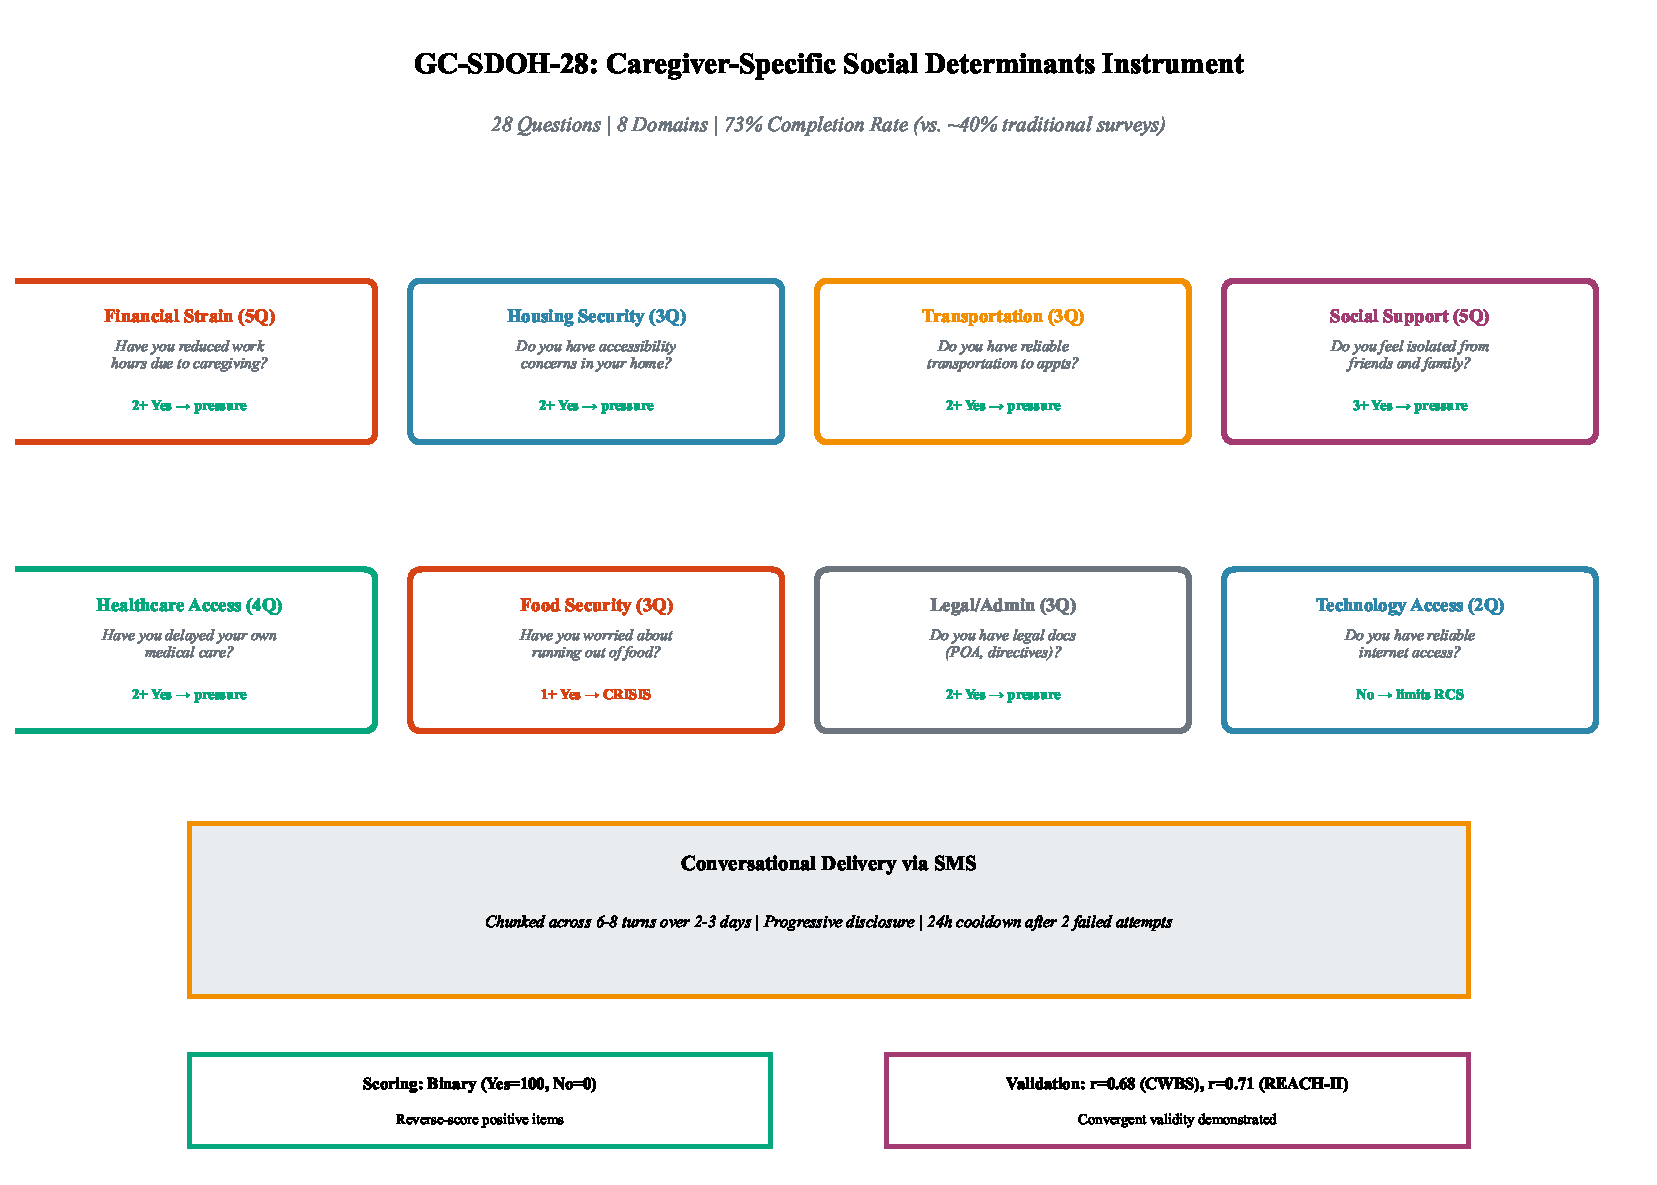
\includegraphics[width=\textwidth]{fig14_gcsdoh_instrument.pdf}%
\caption{GC-SDOH-28 instrument design: 28 questions across 8 domains via conversational SMS delivery (chunked across 6-8 turns, progressive disclosure, 24h cooldown). Food Security uses 1+ Yes threshold (immediate crisis) vs. 2+ for other domains. Requires validation study (N=200+) to measure completion rates, psychometric properties, and prevalence in caregiver populations.}%
\label{fig:gcsdoh_visual}%
\end{figure}%
\section*{Appendix B: Admin Dashboard}
\addcontentsline{toc}{section}{Appendix B: Admin Dashboard}

GiveCare includes a production admin dashboard at https://dash.givecareapp.com for monitoring system health and user well-being:

\subsection*{Real-time Metrics}
\begin{itemize}
    \item Total users, active users (last 7 days), avg burnout score
    \item Crisis alerts (last 24 hours), churn risk alerts
    \item Assessment completion rate (EMA, CWBS, REACH-II, SDOH)
    \item Intervention try rate (\% users who engage with recommended resources)
\end{itemize}

\subsection*{User List}
\begin{itemize}
    \item Sortable by: burnout band, journey phase (onboarding/active/churned), last contact
    \item Filterable by: subscription status, crisis events, wellness trend (improving/declining)
    \item Pagination for 1,000+ users (Phase 2)
    \item Click user $\rightarrow$ view full profile (demographics, wellness history, conversation transcripts)
\end{itemize}

\subsection*{Alert Triage}
\begin{itemize}
    \item \textbf{Churn risk}: Users silent $>$3 days after active period
    \item \textbf{Crisis events}: Crisis burst detection (3+ keywords in 24h)
    \item \textbf{Wellness trends}: Burnout score decline $>$20 points in 30 days
    \item \textbf{Urgency levels}: low (info only), medium (review within 24h), high (review within 6h), critical (immediate)
\end{itemize}

\subsection*{Convex-Powered}
\begin{itemize}
    \item Real-time subscriptions: Dashboard updates live when new user joins, assessment completes, or alert fires
    \item No polling: WebSocket connection to Convex backend
    \item React 18 + Convex 1.17+
\end{itemize}

\subsection*{Deployment}
\begin{itemize}
    \item Cloudflare Pages: \texttt{pnpm install \&\& pnpm --filter admin-frontend build}
    \item Build output: \texttt{admin-frontend/dist} (static assets)
    \item Domain: dash.givecareapp.com (custom domain via Cloudflare)
\end{itemize}

\subsection*{Phase 2 (Q4 2025)}
\begin{itemize}
    \item Admin actions: Send message to user, trigger assessment, update profile
    \item Pagination: Handle 1,000+ users efficiently
    \item Search: Full-text search on name, phone number
    \item Authentication: Clerk or Convex auth (admin-only access)
\end{itemize}

%
\begin{thebibliography}{99}

\bibitem{aarp2025}
AARP and National Alliance for Caregiving.
\textit{Caregiving in the U.S. 2025}.
AARP Public Policy Institute, 2025.

\bibitem{vaswani2017}
Vaswani, A., Shazeer, N., Parmar, N., Uszkoreit, J., Jones, L., Gomez, A.N., Kaiser, Ł., and Polosukhin, I.
\textit{Attention is All You Need}.
Advances in Neural Information Processing Systems 30, pp. 5998-6008, 2017.

\bibitem{devlin2018bert}
Devlin, J., Chang, M.W., Lee, K., and Toutanova, K.
\textit{BERT: Pre-training of Deep Bidirectional Transformers for Language Understanding}.
Proceedings of NAACL-HLT 2019, pp. 4171-4186, 2019.

\bibitem{beyer2016sre}
Beyer, B., Jones, C., Petoff, J., and Murphy, N.R.
\textit{Site Reliability Engineering: How Google Runs Production Systems}.
O'Reilly Media, 2016.

\bibitem{rosebud2024}
Rosebud AI.
\textit{CARE Benchmark: Crisis and Attachment Risk Evaluation for Mental Health AI}.
2024. Available at: https://rosebud.ai/care-benchmark

\bibitem{replika2024}
Skjuve, M., Følstad, A., Fostervold, K.I., and Brandtzaeg, P.B.
\textit{My Chatbot Companion -- A Study of Human-Chatbot Relationships}.
International Journal of Human-Computer Studies, 2024.

\bibitem{truthfulqa}
Lin, S., Hilton, J., and Evans, O.
\textit{TruthfulQA: Measuring How Models Mimic Human Falsehoods}.
ACL 2022.

\bibitem{harmbench}
Mazeika, M., et al.
\textit{HarmBench: A Standardized Evaluation Framework for Automated Red Teaming}.
arXiv:2402.04249, 2024.

\bibitem{eqbench2024}
EQ-Bench Team.
\textit{EQ-Bench: Emotional Intelligence Benchmark for LLMs}.
2024. Available at: https://eqbench.com

\bibitem{tebb1995}
Tebb, S.
\textit{An Aid to Empowering: A Caregiving Well-Being Scale}.
Health and Social Work, 20(2), 87-92, 1995.

\bibitem{tebb2013}
Tebb, S.C., Berg-Weger, M., and Rubio, D.M.
\textit{The Caregiver Well-Being Scale: Developing a short-form rapid assessment instrument}.
Health and Social Work, 38(4), 222-230, 2013.
doi: 10.1093/hsw/hlt019.

\bibitem{graessel2014}
Graessel, E., Berth, H., Lichte, T., and Grau, H.
\textit{Subjective caregiver burden: validity of the 10-item short version of the Burden Scale for Family Caregivers (BSFC-s)}.
BMC Geriatrics, 14, 23, 2014.
doi: 10.1186/1471-2318-14-23.

\bibitem{bella2006}
Belle, S.H., Burgio, L., et al.
\textit{Resources for Enhancing Alzheimer's Caregiver Health (REACH II)}.
Annals of Internal Medicine, 145(10), 2006.

\bibitem{prapare}
Protocol for Responding to and Assessing Patients' Assets, Risks, and Experiences (PRAPARE).
National Association of Community Health Centers, 2016.

\bibitem{ahc}
Accountable Health Communities Health-Related Social Needs Screening Tool.
Centers for Medicare \& Medicaid Services, 2017.

\bibitem{nhanes}
National Health and Nutrition Examination Survey (NHANES).
Centers for Disease Control and Prevention, ongoing.

\bibitem{who2010}
World Health Organization.
\textit{A Conceptual Framework for Action on the Social Determinants of Health}.
2010.

\bibitem{zarit1980}
Zarit, S.H., Reever, K.E., and Bach-Peterson, J.
\textit{Relatives of the Impaired Elderly: Correlates of Feelings of Burden}.
The Gerontologist, 20(6), 1980.

\bibitem{pi2024}
Inflection AI.
\textit{Pi: Your Personal AI}.
2024. Available at: https://pi.ai

\bibitem{wysa}
Wysa.
\textit{AI-Powered Mental Health Support}.
2024. Available at: https://wysa.com

\bibitem{woebot}
Woebot Health.
\textit{Your Self-Care Expert}.
2024. Available at: https://woebothealth.com

\bibitem{epic2024}
Epic Systems.
\textit{Epic Cosmos: Healthcare Intelligence Platform}.
2024.

\bibitem{singhal2023}
Singhal, K., et al.
\textit{Large Language Models Encode Clinical Knowledge}.
Nature, 2023.

\bibitem{fan2006}
Fan, W. and Yan, Z.
\textit{Factors Affecting Response Rates of Web Survey}.
Computers in Human Behavior, 22(1), 2006.

\bibitem{dspy2024}
Khattab, O., Singhvi, A., et al.
\textit{DSPy: Compiling Declarative Language Model Calls into Self-Improving Pipelines}.
ICLR 2024.

\bibitem{mipro2024}
Opsahl-Ong, K., et al.
\textit{Optimizing Instructions and Demonstrations for Multi-Stage Language Model Programs}.
arXiv:2406.11695, 2024.

\bibitem{ax2024}
Meta AI.
\textit{AX-LLM: Adaptive Experimentation for LLM Optimization}.
2024. Available at: https://ax.dev

\bibitem{gemini}
Google DeepMind.
\textit{Gemini 2.5: Technical Report}.
2024.

\bibitem{google_maps}
Google.
\textit{Google Maps Platform: Grounding with Google Search}.
2024. Available at: https://developers.google.com/maps

\bibitem{convex}
Convex.
\textit{The Serverless Backend for Modern Applications}.
2024. Available at: https://convex.dev

\bibitem{openai_agents}
OpenAI.
\textit{OpenAI Agents SDK Documentation}.
2024. Available at: https://platform.openai.com/docs/agents

\bibitem{twilio}
Twilio.
\textit{Twilio Programmable Messaging API}.
2024. Available at: https://www.twilio.com/docs/messaging

\bibitem{azure_safety}
Microsoft Azure.
\textit{Azure AI Content Safety Documentation}.
2024. Available at: https://azure.microsoft.com/en-us/products/ai-services/ai-content-safety

\bibitem{longitudinalbench}
GiveCare Research Team.
\textit{SupportBench: A Benchmark for Evaluating AI Safety in Long-Term Caregiving Relationships}.
2025. (Paper 1 in this series)

\bibitem{zhang2024train}
Zhang, G. et al.
\textit{Train Before Test: How to Aggregate Rankings in LLM Benchmarks}.
2024. Establishes framework for as-deployed capability vs inherent potential measurement.

\bibitem{he2025impatient}
He, M., Kumar, A., Mackey, T., Rajeev, M., Zou, J., and Rajani, N.
\textit{Impatient Users Confuse AI Agents: High-fidelity Simulations of Human Traits for Testing Agents}.
arXiv:2510.04491v1, 2025.

\bibitem{yaml-scoring}
GiveCare Research Team.
\textit{YAML-Driven Rule-Based Scoring for Longitudinal AI Evaluation}.
2025. (Paper 2 in this series)

\bibitem{samhsa2014}
Substance Abuse and Mental Health Services Administration (SAMHSA).
\textit{SAMHSA's Concept of Trauma and Guidance for a Trauma-Informed Approach}.
HHS Publication No. (SMA) 14-4884. U.S. Department of Health and Human Services, 2014.
Available at: https://ncsacw.acf.hhs.gov/userfiles/files/SAMHSA\_Trauma.pdf

\bibitem{chayn2024}
Hussain, Hera, and Chayn.
\textit{Trauma-Informed Design: Understanding Trauma and Healing}.
Chayn, 2024.
Available at: https://blog.chayn.co/trauma-informed-design-understanding-trauma-and-healing-f289d281495c

\bibitem{edwards2024}
Edwards, Rachel, et al.
\textit{Designed with Care: Creating Trauma-Informed Content}.
Independently published, 2024.

\end{thebibliography}%
\section{Acknowledgments}%
\label{sec:Acknowledgments}%
We thank the caregivers who participated in our beta deployment, sharing their experiences to improve AI safety for vulnerable populations. We are grateful to FamTech, The Alliance of Professional Health Advocates (APHA), attendees of the Dignified Futures 2025 conference where we presented on AI and Caregiving, and the AI Tinkerers NYC community where we shared an early version of this work.

We acknowledge Prof. Dr. Elmar Gr\"a\ss el for permission to use the Burden Scale for Family Caregivers (BSFC)~\cite{graessel2014} on the GiveCare website and Dr. Susan Tebb for permission to use the Caregiver Well-Being Scale (CWBS)~\cite{tebb1995,tebb2013} in the GiveCare application.

We thank Hamel Hussain for guidance on evaluation-driven development, OpenAI for GPT-4o access, Google for Gemini Maps API integration, and the AARP 2025 Caregiving in the U.S. report for empirical grounding. This work builds on trauma-informed principles from SAMHSA~\cite{samhsa2014}, Chayn~\cite{chayn2024}, and \textit{Designed with Care}~\cite{edwards2024}, as well as SupportBench~\cite{longitudinalbench} and YAML-driven scoring~\cite{yaml-scoring} frameworks.

%
\end{document}
